% =====================================================================
%  Unified Content Authenticity Verification System
%  Project Overview, Algorithms and System Design
%
%  Compile with pdfLaTeX or XeLaTeX (for example on Overleaf).
%  Needs: TikZ, pgfgantt, algorithmicx, adjustbox (all in TeX Live / MiKTeX).
% =====================================================================
\documentclass[11pt,a4paper]{article}

\usepackage[a4paper,margin=2.2cm,headheight=14pt]{geometry}
\usepackage[T1]{fontenc}
\usepackage[utf8]{inputenc}
\usepackage{lmodern}
\usepackage{microtype}
\usepackage{amsmath,amssymb}
\usepackage{xcolor}
\usepackage{booktabs,tabularx,array}
\usepackage{enumitem}
\usepackage{caption}
\usepackage{adjustbox}
\usepackage[section]{placeins}
\usepackage{float}
\usepackage{algorithm}
\usepackage{algpseudocode}
\usepackage{fancyhdr}
\usepackage{tikz}
\usetikzlibrary{shapes.geometric,shapes.multipart,shapes.misc,arrows.meta,positioning,fit,calc,backgrounds}
\usepackage{pgfgantt}

% ---------------------------------------------------------------------
% Colours (indigo / teal palette, same as the presentation deck)
% ---------------------------------------------------------------------
\definecolor{cPrimary}{HTML}{3949AB}
\definecolor{cAccent}{HTML}{00897B}
\definecolor{cRed}{HTML}{D84343}
\definecolor{cAmber}{HTML}{F2A33A}
\definecolor{cGreen}{HTML}{3A9D5D}
\definecolor{cInk}{HTML}{1F2937}
\definecolor{cMuted}{HTML}{6B7280}

\usepackage[colorlinks=true,linkcolor=cPrimary,urlcolor=cAccent,citecolor=cAccent]{hyperref}

% ---------------------------------------------------------------------
% Page style
% ---------------------------------------------------------------------
\pagestyle{fancy}
\fancyhf{}
\fancyhead[L]{\small\color{cMuted}Unified Content Authenticity Verification System}
\fancyhead[R]{\small\color{cMuted}The Perceptrons}
\fancyfoot[C]{\small\thepage}
\renewcommand{\headrulewidth}{0.4pt}

\setlist{itemsep=2pt,topsep=4pt}
\captionsetup{font=small,labelfont={bf,color=cPrimary}}
\renewcommand{\arraystretch}{1.25}
\newcolumntype{Y}{>{\raggedright\arraybackslash}X}

\renewcommand{\algorithmicrequire}{\textbf{Input:}}
\renewcommand{\algorithmicensure}{\textbf{Output:}}

% ---------------------------------------------------------------------
% TikZ styles
% ---------------------------------------------------------------------
\tikzset{
  >={Stealth[length=2.2mm]},
  every node/.append style={execute at begin node={\hyphenpenalty=10000\exhyphenpenalty=10000\relax}},
  flow/.style={->, thick, draw=cInk!80},
  dflow/.style={->, thick, dashed, draw=cMuted},
  block/.style={draw=cPrimary, fill=cPrimary!7, rounded corners=3pt, align=center,
                font=\small, inner sep=5pt, minimum height=9mm},
  ablock/.style={block, draw=cAccent, fill=cAccent!9},
  gblock/.style={block, draw=cMuted, fill=cMuted!10},
  vgood/.style={block, draw=cGreen, fill=cGreen!14},
  vwarn/.style={block, draw=cAmber, fill=cAmber!18},
  vbad/.style={block, draw=cRed, fill=cRed!10},
  startstop/.style={rounded rectangle, draw=cInk, fill=cInk!8, align=center,
                    font=\small\bfseries, minimum height=8mm, minimum width=2.4cm},
  decision/.style={diamond, aspect=2.2, draw=cAccent, fill=cAccent!10, align=center,
                   font=\small, inner sep=1.5pt},
  io/.style={trapezium, trapezium left angle=72, trapezium right angle=108,
             trapezium stretches body, draw=cPrimary, fill=white, align=center,
             font=\small, minimum height=8mm, inner xsep=3pt},
  store/.style={cylinder, shape border rotate=90, aspect=0.22, draw=cAccent,
                fill=cAccent!9, align=center, font=\small, minimum height=1.5cm},
  lbl/.style={font=\footnotesize, text=cMuted, align=center},
  process/.style={circle, draw=cPrimary, fill=cPrimary!7, align=center,
                  font=\small, minimum size=2.3cm, inner sep=1pt},
  entity/.style={rectangle, draw=cInk, fill=cInk!6, align=center,
                 font=\small\bfseries, minimum width=2.2cm, minimum height=1cm},
  datastore/.style={rectangle split, rectangle split horizontal,
                    rectangle split parts=2, draw=cAccent, fill=cAccent!9,
                    font=\small, minimum height=0.8cm},
  umlclass/.style={rectangle split, rectangle split parts=3, draw=cPrimary,
                   fill=white, font=\footnotesize, text width=3.8cm, align=left,
                   inner sep=3pt},
  seqhead/.style={draw=cPrimary, fill=cPrimary!10, rounded corners=2pt,
                  font=\small\bfseries, minimum width=2.1cm, minimum height=8mm,
                  align=center},
  usecase/.style={ellipse, draw=cPrimary, fill=cPrimary!6, font=\small,
                  minimum width=4.6cm, minimum height=0.8cm, align=center},
  actor/.pic={
    \draw[thick, cInk] (0,0.9) circle (0.22);
    \draw[thick, cInk] (0,0.68) -- (0,0.05);
    \draw[thick, cInk] (-0.35,0.45) -- (0.35,0.45);
    \draw[thick, cInk] (0,0.05) -- (-0.28,-0.45);
    \draw[thick, cInk] (0,0.05) -- (0.28,-0.45);
  },
}
\newcommand{\cname}[1]{\makebox[3.8cm][c]{\textbf{#1}}}
\newenvironment{diagram}{\begin{adjustbox}{max totalsize={\linewidth}{0.86\textheight},center}}{\end{adjustbox}}

% =====================================================================
\begin{document}

% ---------------------------------------------------------------------
% Title page
% ---------------------------------------------------------------------
\hypersetup{pageanchor=false}
\begin{titlepage}
\thispagestyle{empty}
\centering
{\color{cPrimary}\rule{\linewidth}{1.2pt}}\par\vspace{1.4em}
{\small\color{cAccent}\textsc{Final Year Project \quad\textbar\quad BE Computer Engineering}}\par\vspace{1.2em}
{\LARGE\bfseries Unified Content Authenticity\\[0.2em] Verification System\par}
\vspace{0.8em}
{\large Deepfake Detection with Cross-Generator Generalization\\ and Document Tamper Localization\par}
\vspace{1.2em}
{\Large\color{cPrimary} Project Overview, Algorithms and System Design\par}
\vspace{1.2em}
{\color{cPrimary}\rule{\linewidth}{1.2pt}}\par
\vfill
{\large\bfseries Team: The Perceptrons\par}
\vspace{0.6em}
Pawan Singh Jagdish Bhandari\\
Rahul H.\ Bramhankar\\
Bhoomi Kushwah\par
\vspace{1.4em}
{\bfseries Project Guide:} Dr.\ Gayatri Bhandari (HOD)\par
\vspace{1.4em}
Department of Computer Engineering\\
JSPM's Bhivarabai Sawant Institute of Technology and Research (BSIOTR), Wagholi, Pune\par
\vfill
{\small\color{cMuted} Version 1.0 \quad\textbar\quad September 2026 \quad\textbar\quad Design baseline, written before implementation.\\
Results sections will be filled in as each phase is completed.\par}
\end{titlepage}
\hypersetup{pageanchor=true}

\tableofcontents
\clearpage
\listoffigures
\listofalgorithms
\clearpage

% =====================================================================
\section{Project Overview}
\label{sec:overview}
% =====================================================================

\subsection{The problem}
Generative AI tools such as Stable Diffusion, Midjourney, DALL-E and FLUX now produce images
and videos that people cannot tell apart from real camera footage. At the same time, ordinary
editing tools make it easy to change the amount on an invoice, a date on a contract or a name
on an identity document. Both are used for misinformation, identity theft and financial fraud.

Existing detectors have two main weaknesses:
\begin{enumerate}
  \item \textbf{They do not generalize.} A detector trained on one generator usually fails on
        new ones. A 2026 benchmark of 16 open-source detectors found that mean accuracy falls
        from about 79\% on 2020--21 generators to about 38\% on 2024 generators~\cite{outofbox2026},
        and on deepfakes collected from the internet in 2024 the AUC of open-source detectors
        dropped by roughly half~\cite{deepfakeeval2024}.
  \item \textbf{They do not explain.} Most tools give a bare ``real'' or ``fake'' label, and most
        document checkers do not show \emph{where} a document was edited.
\end{enumerate}

\subsection{What the system does}
A user uploads an \textbf{image}, a \textbf{video} or a \textbf{document}. The system returns:
\begin{enumerate}
  \item a \textbf{Trust Score} $T$ from 0 to 100, where 100 means ``looks authentic'';
  \item a \textbf{verdict}: \emph{Likely Authentic}, \emph{Needs Human Review} or \emph{Likely Manipulated};
  \item \textbf{evidence}: a heatmap or highlighted regions, a list of the signals that were found,
        and a short explanation in plain language.
\end{enumerate}

\subsection{Core idea: cross-generator generalization}
Each AI generator leaves its own ``fingerprint'' of artifacts. A detector that memorizes one
fingerprint is useless against the next generator. Our detector is trained on \emph{one}
generator and is always tested on generators it has \emph{never seen}
(Figure~\ref{fig:concept}). To do this, we rely on features that are shared by many generators:
general visual features from a large pretrained encoder (CLIP), and forensic traces such as
frequency-domain artifacts and noise inconsistencies. The same principle is applied to
documents, where the ``unseen generators'' are new tampering methods and real human-made
forgeries.

\begin{figure}[htbp]
\centering
\begin{diagram}
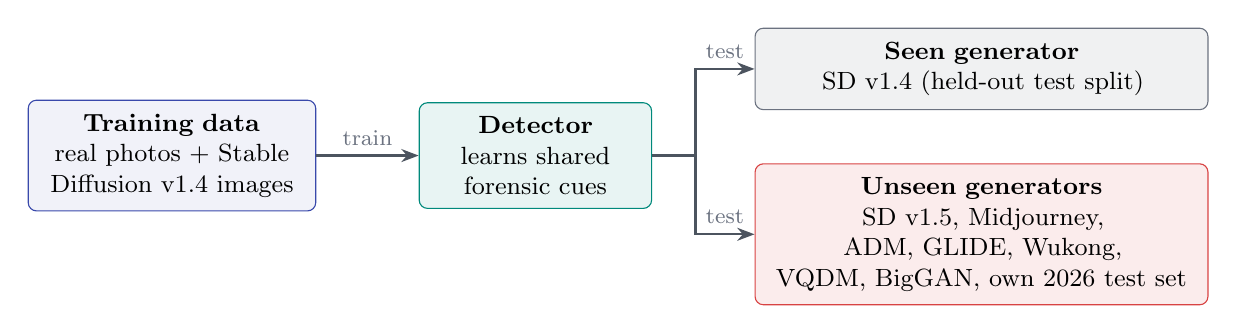
\begin{tikzpicture}
  \node[block, text width=3.3cm] (train) {\textbf{Training data}\\ real photos + Stable Diffusion v1.4 images};
  \node[ablock, text width=2.6cm, right=1.3cm of train] (det) {\textbf{Detector}\\ learns shared forensic cues};
  \node[gblock, text width=5.4cm, right=1.3cm of det, yshift=1.1cm] (seen) {\textbf{Seen generator}\\ SD v1.4 (held-out test split)};
  \node[vbad, text width=5.4cm, right=1.3cm of det, yshift=-1.0cm] (unseen) {\textbf{Unseen generators}\\ SD v1.5, Midjourney, ADM, GLIDE, Wukong,\\ VQDM, BigGAN, own 2026 test set};
  \draw[flow] (train) -- node[lbl, above]{train} (det);
  \draw[flow] (det.east) -- ++(0.55,0) |- node[lbl, pos=0.75, above]{test} (seen.west);
  \draw[flow] (det.east) -- ++(0.55,0) |- node[lbl, pos=0.75, above]{test} (unseen.west);
\end{tikzpicture}
\end{diagram}
\caption{Cross-generator generalization: train on one generator, test on many unseen ones.}
\label{fig:concept}
\end{figure}

\subsection{Three phases}
The project is built one content type at a time. Each phase ends with a working demo, and each
later phase reuses the Trust Scoring Engine and web app built in Phase~1.

\begin{table}[htbp]
\centering
\small
\begin{tabularx}{\linewidth}{@{}l Y Y Y Y@{}}
\toprule
\textbf{Phase} & \textbf{Detects} & \textbf{Main algorithm} & \textbf{Training data} & \textbf{``Unseen'' test} \\
\midrule
1 --- Image & Fully AI-generated images & Frozen CLIP encoder + frequency features + logistic head & GenImage: real + SD v1.4 & 7 other GenImage generators + own 2026 test set \\
2 --- Video & Face-swapped / re-enacted videos & Face detection + frame classifier + temporal aggregation & FaceForensics++ & Celeb-DF v2 \\
3 --- Document & Edited regions in documents & Dual-stream U-Net + OCR logic checks + PDF checks & Own synthetic forgeries & Real human-made forgeries (RTM) \\
\bottomrule
\end{tabularx}
\caption{The three phases at a glance.}
\label{tab:phases}
\end{table}

\subsection{Scope}
\textbf{In scope:} still images, short videos with faces (and full-frame analysis for videos
without faces), scanned or photographed documents and PDFs; a calibrated Trust Score; visual and
written explanations; a Streamlit web demo.

\textbf{Out of scope:} audio deepfakes, real-time video streams, legal-grade certification,
training large multimodal language models.

\subsection{Planned contributions}
\begin{enumerate}
  \item Cross-generator generalization measured in \emph{every} phase, including a self-built
        test set of recent (2026) generators.
  \item A \textbf{calibrated} Trust Score with a \emph{Needs Human Review} band chosen to keep
        the error rate of automatic decisions under a target.
  \item Evidence-grounded explanations: heatmaps, frequency evidence, OCR logic checks and file
        metadata, turned into plain-language sentences.
  \item Evaluation that controls for known dataset shortcuts (JPEG format and image size) and
        tests robustness to compression, resizing and blur.
\end{enumerate}
Related work already unifies these forensic domains as a research benchmark
(ForensicHub~\cite{forensichub}); our focus is an end-user system that is explainable,
calibrated and tested on unseen generators.

% =====================================================================
\section{System Architecture}
\label{sec:architecture}
% =====================================================================

\subsection{Architecture overview}
Figure~\ref{fig:architecture} shows the complete system. It has five layers:
\begin{enumerate}
  \item \textbf{Presentation layer:} the Streamlit web interface where users upload files and read reports.
  \item \textbf{Routing layer:} validates the file and sends it to the correct pipeline.
  \item \textbf{Analysis layer:} three independent pipelines (image, video, document). Each
        returns the same kind of \texttt{Evidence} object (Section~\ref{sec:evidence-object}).
  \item \textbf{Decision layer:} evidence fusion, calibration and the Unified Trust Scoring Engine.
  \item \textbf{Reporting layer:} builds the report with score, verdict, heatmaps and explanation.
\end{enumerate}
Models are trained \emph{offline} on free GPUs (Google Colab / Kaggle). The trained weights and
calibration parameters are saved to a \emph{model store} that the pipelines load at run time.

\begin{figure}[htbp]
\centering
\begin{diagram}
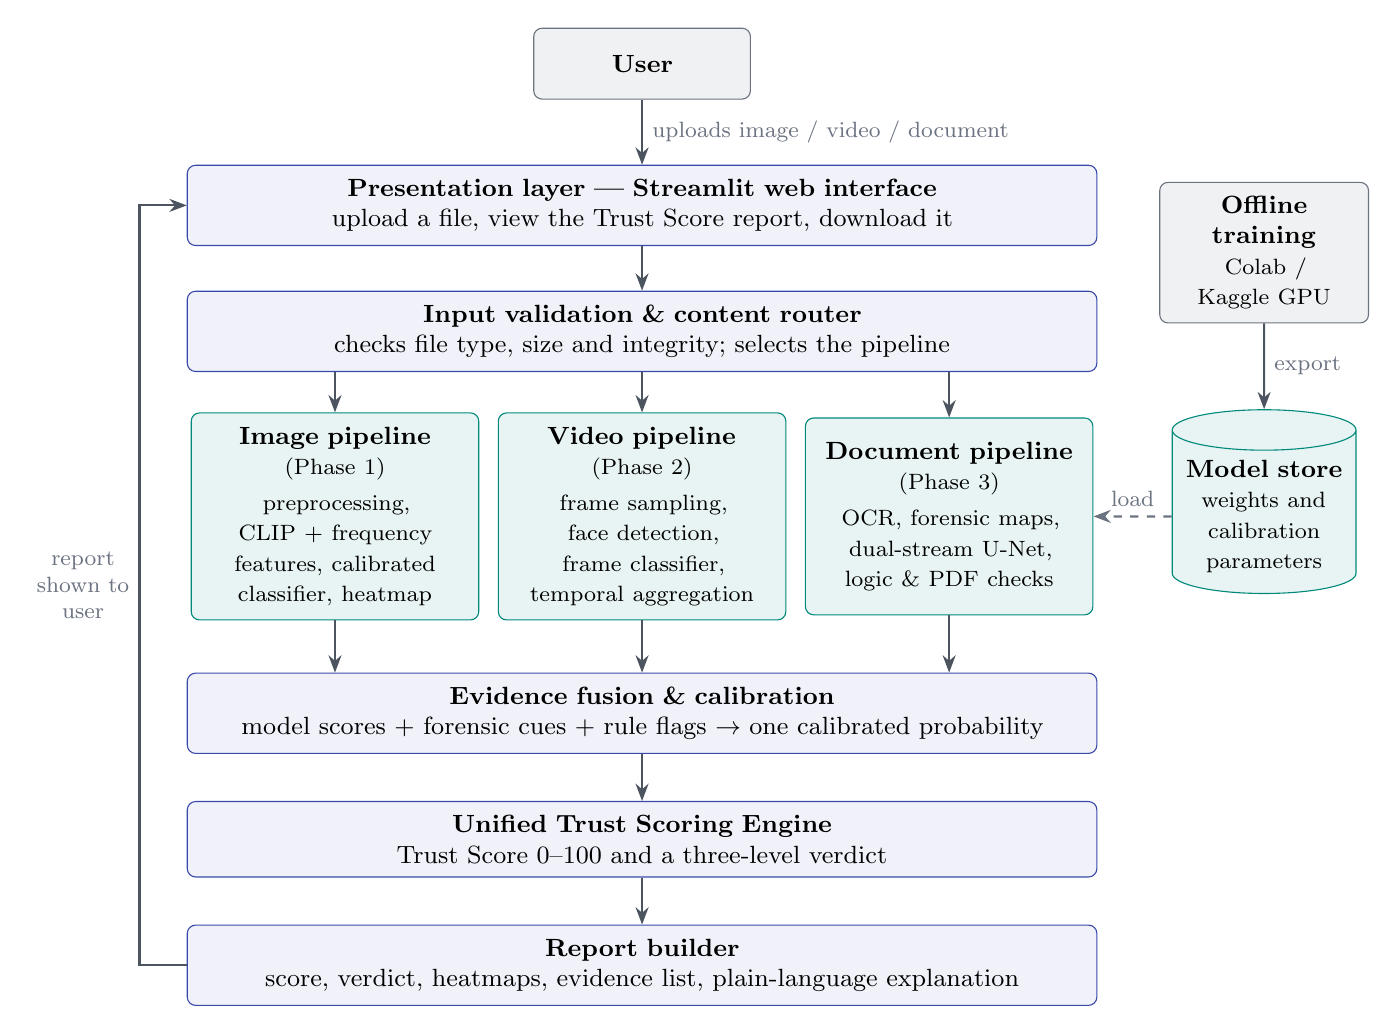
\begin{tikzpicture}
  \node[gblock, text width=2.4cm] (user) at (5.8,1.8) {\textbf{User}};
  \node[block, text width=11.2cm] (ui) at (5.8,0) {\textbf{Presentation layer --- Streamlit web interface}\\ upload a file, view the Trust Score report, download it};
  \node[block, text width=11.2cm] (router) at (5.8,-1.6) {\textbf{Input validation \& content router}\\ checks file type, size and integrity; selects the pipeline};
  \node[ablock, text width=3.3cm, minimum height=2.5cm] (img) at (1.9,-3.95) {\textbf{Image pipeline}\\ {\footnotesize (Phase 1)}\\[2pt] {\footnotesize preprocessing, CLIP + frequency features, calibrated classifier, heatmap}};
  \node[ablock, text width=3.3cm, minimum height=2.5cm] (vid) at (5.8,-3.95) {\textbf{Video pipeline}\\ {\footnotesize (Phase 2)}\\[2pt] {\footnotesize frame sampling, face detection, frame classifier, temporal aggregation}};
  \node[ablock, text width=3.3cm, minimum height=2.5cm] (doc) at (9.7,-3.95) {\textbf{Document pipeline}\\ {\footnotesize (Phase 3)}\\[2pt] {\footnotesize OCR, forensic maps, dual-stream U-Net, logic \& PDF checks}};
  \node[block, text width=11.2cm] (fuse) at (5.8,-6.45) {\textbf{Evidence fusion \& calibration}\\ model scores + forensic cues + rule flags $\rightarrow$ one calibrated probability};
  \node[block, text width=11.2cm] (trust) at (5.8,-8.05) {\textbf{Unified Trust Scoring Engine}\\ Trust Score 0--100 and a three-level verdict};
  \node[block, text width=11.2cm] (report) at (5.8,-9.65) {\textbf{Report builder}\\ score, verdict, heatmaps, evidence list, plain-language explanation};
  \node[store, text width=2.1cm] (models) at (13.7,-3.95) {\textbf{Model store}\\ {\footnotesize weights and calibration parameters}};
  \node[gblock, text width=2.3cm] (train) at (13.7,-0.6) {\textbf{Offline training}\\ {\footnotesize Colab / Kaggle GPU}};

  \draw[flow] (user) -- node[lbl, right]{uploads image / video / document} (ui);
  \draw[flow] (ui) -- (router);
  \foreach \n in {img,vid,doc} {
    \draw[flow] (router.south -| \n.north) -- (\n.north);
    \draw[flow] (\n.south) -- (\n.south |- fuse.north);
  }
  \draw[flow] (fuse) -- (trust);
  \draw[flow] (trust) -- (report);
  \draw[flow] (report.west) -- ++(-0.6,0) |- node[lbl, pos=0.25, left]{report\\shown to\\user} (ui.west);
  \draw[flow] (train) -- node[lbl, right]{export} (models);
  \draw[dflow] (models.west) -- node[lbl, above]{load} (doc.east);
\end{tikzpicture}
\end{diagram}
\caption{High-level system architecture. All three pipelines load their weights from the model store.}
\label{fig:architecture}
\end{figure}

\subsection{Design principles}
\begin{itemize}
  \item \textbf{One common interface.} Every pipeline returns an \texttt{Evidence} object, so the
        Trust Scoring Engine and the report builder do not depend on the content type. New
        pipelines can be added without changing them.
  \item \textbf{Training is separate from inference.} Heavy training runs on free cloud GPUs; the
        web app only loads saved weights and runs on a normal laptop CPU.
  \item \textbf{Calibration is its own step.} Raw model outputs are not probabilities. Every
        pipeline is calibrated on validation data before its score is used.
  \item \textbf{Explanations are required.} No verdict is shown without the evidence behind it.
  \item \textbf{Reproducibility.} Fixed random seeds, written data cards, saved train/validation/test
        split lists and an experiment log.
\end{itemize}

\subsection{End-to-end processing flow}
Figure~\ref{fig:flowchart} shows what happens from the moment a user uploads a file until the
report is shown.

\begin{figure}[p]
\centering
\begin{diagram}
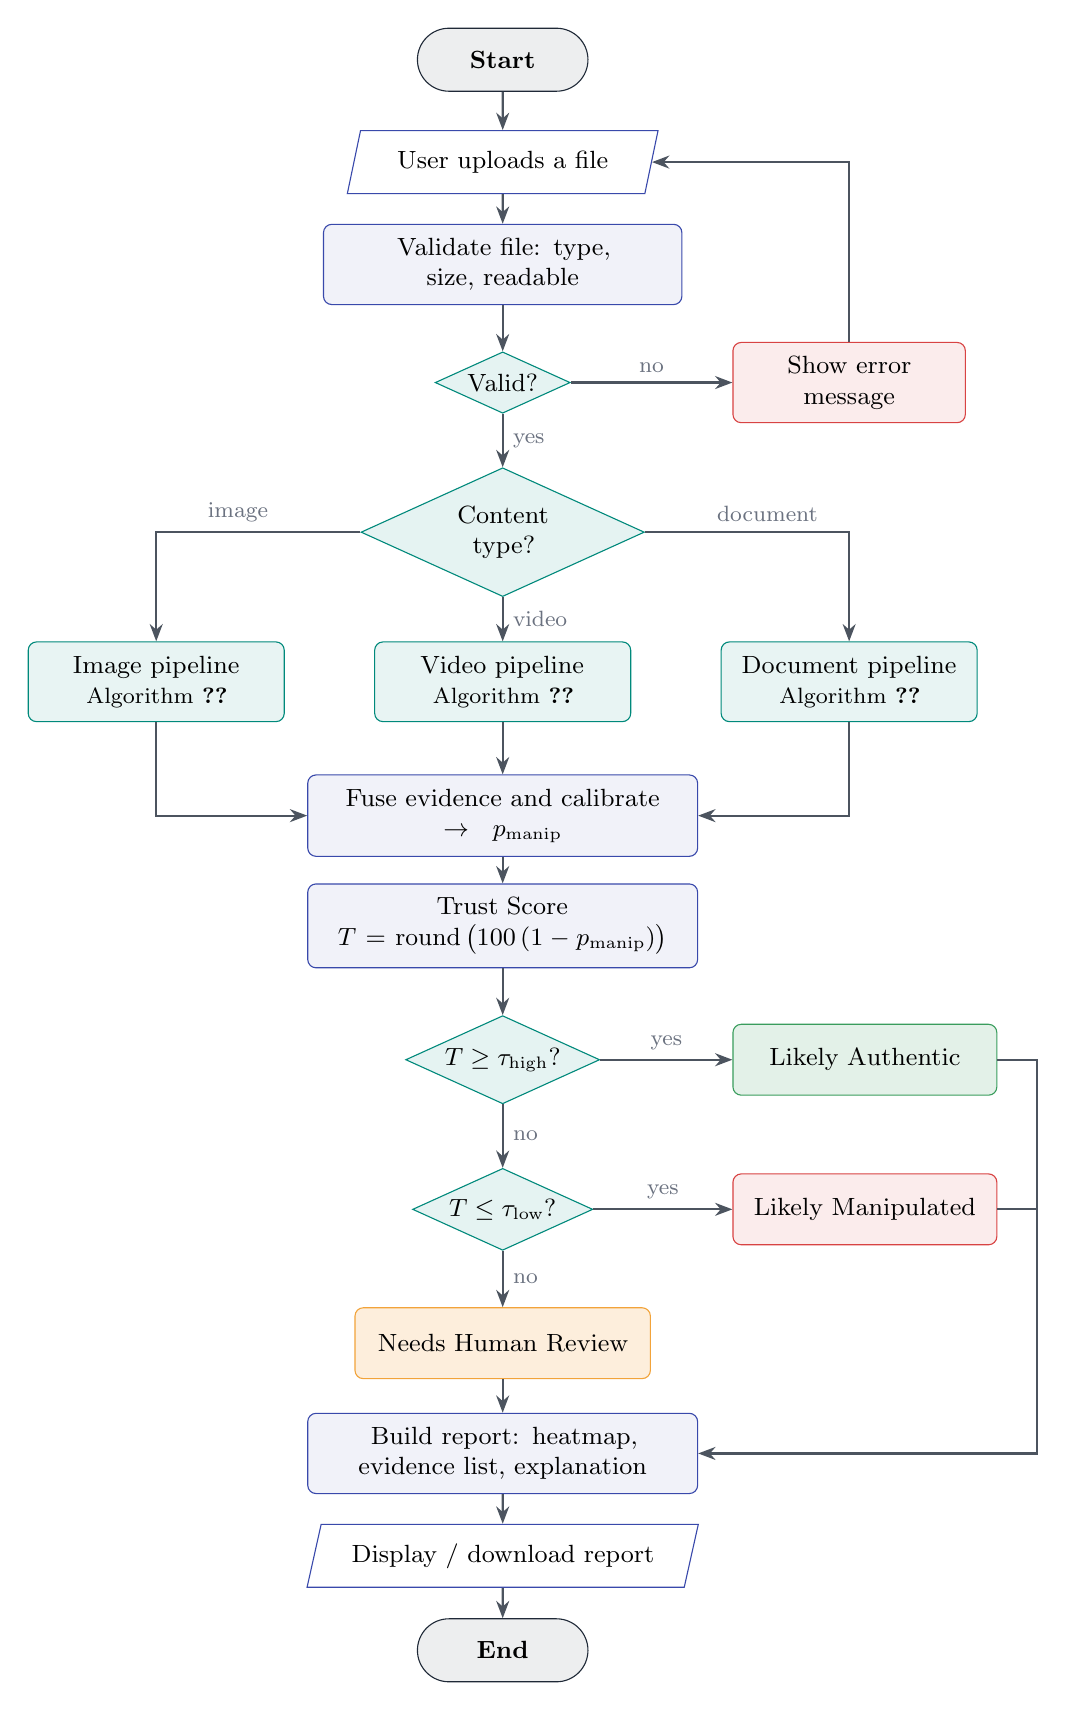
\begin{tikzpicture}
  \node[startstop] (start) at (0,0) {Start};
  \node[io, text width=3.4cm] (upload) at (0,-1.3) {User uploads a file};
  \node[block, text width=4.2cm] (validate) at (0,-2.6) {Validate file: type, size, readable};
  \node[decision] (valid) at (0,-4.1) {Valid?};
  \node[vbad, text width=2.6cm] (err) at (4.4,-4.1) {Show error message};
  \node[decision, text width=1.8cm] (type) at (0,-6.0) {Content type?};
  \node[ablock, text width=2.9cm] (img) at (-4.4,-7.9) {Image pipeline\\ {\footnotesize Algorithm~\ref{alg:image-infer}}};
  \node[ablock, text width=2.9cm] (vid) at (0,-7.9) {Video pipeline\\ {\footnotesize Algorithm~\ref{alg:video}}};
  \node[ablock, text width=2.9cm] (doc) at (4.4,-7.9) {Document pipeline\\ {\footnotesize Algorithm~\ref{alg:doc-infer}}};
  \node[block, text width=4.6cm] (fuse) at (0,-9.6) {Fuse evidence and calibrate\\ $\rightarrow p_{\text{manip}}$};
  \node[block, text width=4.6cm] (score) at (0,-11.0) {Trust Score\\ $T=\operatorname{round}\big(100\,(1-p_{\text{manip}})\big)$};
  \node[decision] (d1) at (0,-12.7) {$T\ge\tau_{\text{high}}$?};
  \node[vgood, text width=3.0cm] (auth) at (4.6,-12.7) {Likely Authentic};
  \node[decision] (d2) at (0,-14.6) {$T\le\tau_{\text{low}}$?};
  \node[vbad, text width=3.0cm] (manip) at (4.6,-14.6) {Likely Manipulated};
  \node[vwarn, text width=3.4cm] (review) at (0,-16.3) {Needs Human Review};
  \node[block, text width=4.6cm] (report) at (0,-17.7) {Build report: heatmap, evidence list, explanation};
  \node[io, text width=4.4cm] (show) at (0,-19.0) {Display / download report};
  \node[startstop] (stop) at (0,-20.2) {End};

  \draw[flow] (start) -- (upload);
  \draw[flow] (upload) -- (validate);
  \draw[flow] (validate) -- (valid);
  \draw[flow] (valid) -- node[lbl, above]{no} (err);
  \draw[flow] (err.north) |- (upload.east);
  \draw[flow] (valid) -- node[lbl, right]{yes} (type);
  \draw[flow] (type.west) -| node[lbl, pos=0.3, above]{image} (img.north);
  \draw[flow] (type.south) -- node[lbl, right]{video} (vid.north);
  \draw[flow] (type.east) -| node[lbl, pos=0.3, above]{document} (doc.north);
  \draw[flow] (img.south) |- (fuse.west);
  \draw[flow] (vid.south) -- (fuse.north);
  \draw[flow] (doc.south) |- (fuse.east);
  \draw[flow] (fuse) -- (score);
  \draw[flow] (score) -- (d1);
  \draw[flow] (d1) -- node[lbl, above]{yes} (auth);
  \draw[flow] (d1) -- node[lbl, right]{no} (d2);
  \draw[flow] (d2) -- node[lbl, above]{yes} (manip);
  \draw[flow] (d2) -- node[lbl, right]{no} (review);
  \draw[flow] (review) -- (report);
  \draw[flow] (auth.east) -- ++(0.5,0) |- (report.east);
  \draw[thick, draw=cInk!80] (manip.east) -- ++(0.5,0);
  \draw[flow] (report) -- (show);
  \draw[flow] (show) -- (stop);
\end{tikzpicture}
\end{diagram}
\caption{End-to-end processing flowchart.}
\label{fig:flowchart}
\end{figure}

\subsection{Module decomposition}

\begin{table}[htbp]
\centering
\small
\begin{tabularx}{\linewidth}{@{}l Y Y Y@{}}
\toprule
\textbf{Module} & \textbf{Input} & \textbf{Output} & \textbf{Main technique} \\
\midrule
Web interface & File from the user & Rendered report & Streamlit \\
Content router & Uploaded file & Content type, validated file & MIME type, extension, decoding test \\
Image analyzer & Image & \texttt{Evidence} (probability, heatmap, spectrum score) & CLIP features, radial FFT spectrum, logistic head \\
Video analyzer & Video & \texttt{Evidence} (probability, frame timeline, heatmaps) & Frame sampling, MTCNN, frame classifier, top-$k$ aggregation \\
Document analyzer & Scan, photo or PDF & \texttt{Evidence} (localization score, mask, rule flags) & OCR, ELA / SRM / DCT maps, dual-stream U-Net, rule checks \\
Trust Scoring Engine & \texttt{Evidence} & Trust Score $T$, verdict & Logistic fusion, calibration, selective thresholds \\
Report builder & $T$, verdict, \texttt{Evidence} & Report (screen and PDF) & Templates \\
Training \& evaluation & Datasets & Weights, calibration files, results tables & PyTorch, scikit-learn \\
\bottomrule
\end{tabularx}
\caption{System modules.}
\label{tab:modules}
\end{table}

% =====================================================================
\section{Phase 1: Image Authenticity Algorithms}
\label{sec:image}
% =====================================================================

\subsection{Pipeline}
The image pipeline (Figure~\ref{fig:image-pipeline}) has two feature branches: a \emph{semantic}
branch that uses a frozen CLIP encoder, and a \emph{forensic} branch that measures
frequency-domain artifacts. Their features are joined and passed to a small classifier whose
output is calibrated into a probability.

\begin{figure}[htbp]
\centering
\begin{diagram}
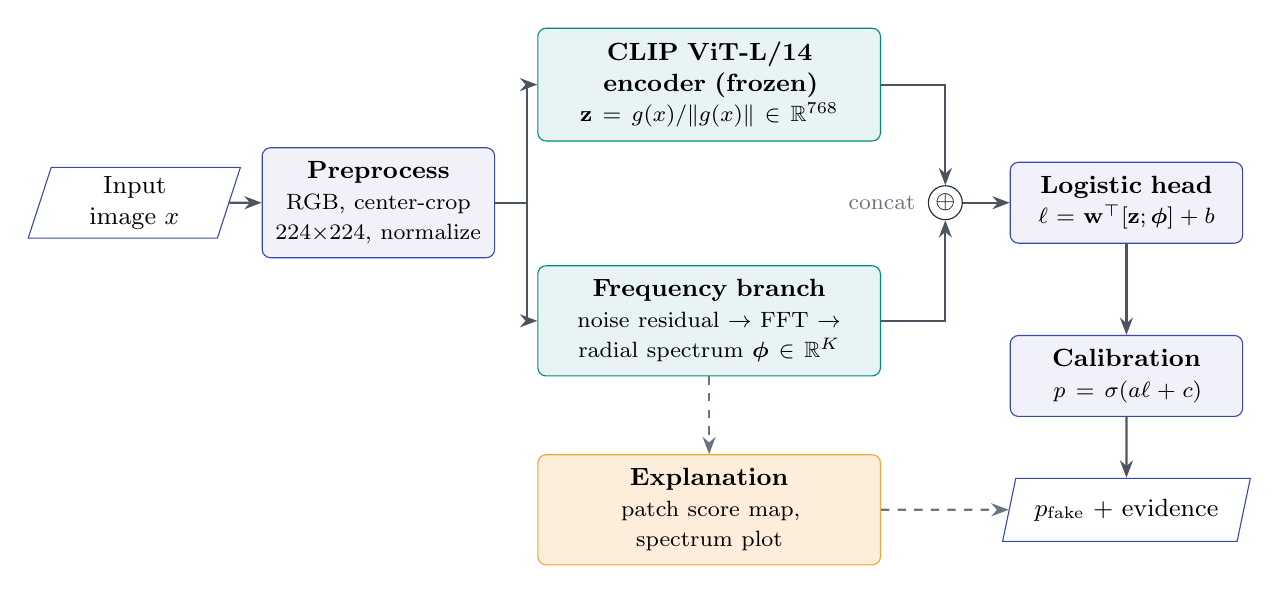
\begin{tikzpicture}
  \node[io, text width=1.9cm] (in) at (0,0) {Input image $x$};
  \node[block, text width=2.6cm] (prep) at (3.1,0) {\textbf{Preprocess}\\ {\footnotesize RGB, center-crop $224{\times}224$, normalize}};
  \node[ablock, text width=4.0cm] (clip) at (7.3,1.5) {\textbf{CLIP ViT-L/14 encoder (frozen)}\\ {\footnotesize $\mathbf{z}=g(x)/\lVert g(x)\rVert\in\mathbb{R}^{768}$}};
  \node[ablock, text width=4.0cm] (freq) at (7.3,-1.5) {\textbf{Frequency branch}\\ {\footnotesize noise residual $\rightarrow$ FFT $\rightarrow$ radial spectrum $\boldsymbol{\phi}\in\mathbb{R}^{K}$}};
  \node[circle, draw=cInk, fill=white, inner sep=1pt, font=\small] (cat) at (10.3,0) {$\oplus$};
  \node[block, text width=2.6cm] (head) at (12.6,0) {\textbf{Logistic head}\\ {\footnotesize $\ell=\mathbf{w}^\top[\mathbf{z};\boldsymbol{\phi}]+b$}};
  \node[block, text width=2.6cm] (cal) at (12.6,-2.2) {\textbf{Calibration}\\ {\footnotesize $p=\sigma(a\ell+c)$}};
  \node[vwarn, text width=4.0cm] (expl) at (7.3,-3.9) {\textbf{Explanation}\\ {\footnotesize patch score map, spectrum plot}};
  \node[io, text width=2.6cm] (out) at (12.6,-3.9) {$p_{\text{fake}}$ + evidence};

  \draw[flow] (in) -- (prep);
  \draw[flow] (prep.east) -- ++(0.4,0) |- (clip.west);
  \draw[flow] (prep.east) -- ++(0.4,0) |- (freq.west);
  \draw[flow] (clip.east) -| (cat.north);
  \draw[flow] (freq.east) -| (cat.south);
  \node[lbl, left=1pt of cat] {concat};
  \draw[flow] (cat) -- (head);
  \draw[flow] (head) -- (cal);
  \draw[flow] (cal) -- (out);
  \draw[dflow] (freq) -- (expl);
  \draw[dflow] (expl) -- (out);
\end{tikzpicture}
\end{diagram}
\caption{Phase 1 image pipeline.}
\label{fig:image-pipeline}
\end{figure}

\subsection{Preprocessing and removing dataset shortcuts}
Public datasets often store real photos as JPEG and generated images as PNG, and generated
images come in a few fixed sizes. A detector can then learn ``JPEG means real'' instead of
learning real generation artifacts. Removing these biases on GenImage improved cross-generator
accuracy by more than 11 percentage points~\cite{fakeorjpeg}. We therefore:
\begin{enumerate}
  \item re-save \emph{all} training images (real and fake) with the same JPEG quality and the same
        crop size;
  \item add random JPEG compression (quality 60--100) during training so the model cannot rely on
        compression traces;
  \item use \textbf{center-cropping} instead of resizing, because resizing blurs away the
        high-frequency traces we want to detect.
\end{enumerate}

\subsection{Baseline: EfficientNet-B0 with transfer learning}
EfficientNet~\cite{efficientnet} scales network depth $d$, width $w$ and input resolution $r$
together with one coefficient $\varphi$:
\begin{equation}
  d=\alpha^{\varphi},\quad w=\beta^{\varphi},\quad r=\gamma^{\varphi},
  \qquad \alpha\cdot\beta^{2}\cdot\gamma^{2}\approx 2,
\end{equation}
with $\alpha=1.2$, $\beta=1.1$, $\gamma=1.15$. EfficientNet-B0 ($\varphi=0$) has about 5.3 million
parameters, which makes it practical on free GPUs. We start from ImageNet weights, replace the
final layer with a single output, and fine-tune the whole network with binary cross-entropy
(Equation~\ref{eq:bce}). This is our \textbf{baseline}: fully fine-tuned CNNs are known to fit the
artifacts of the training generator and generalize poorly, which is exactly the gap our main
model must close.

\subsection{Main model: frozen CLIP encoder with a linear head}
CLIP~\cite{clip} is a vision transformer trained on about 400 million image--text pairs. Its image
features describe general visual properties rather than the quirks of one generator. Ojha
et~al.~\cite{ojha} showed that a simple linear classifier on \emph{frozen} CLIP features detects
images from unseen generators far better than a fully trained CNN.

For an image $x$, the frozen encoder $g$ (ViT-L/14, $224{\times}224$ input split into $16{\times}16$
patches of $14{\times}14$ pixels) gives the normalized embedding
\begin{equation}
  \mathbf{z}=\frac{g(x)}{\lVert g(x)\rVert_2}\in\mathbb{R}^{768}.
\end{equation}
Because $g$ is frozen, embeddings are computed \emph{once} and cached to disk. Training the head
then takes minutes, even on a CPU.

\textbf{Planned upgrade:} fine-tune only the LayerNorm parameters of the encoder (about 0.03\% of
all parameters), which recent work reports generalizes well across 14 deepfake
benchmarks~\cite{gend}.

\subsection{Forensic branch: frequency features}
Generators build images by repeated up-sampling, which leaves periodic patterns that are
invisible in the image but clear in its frequency spectrum~\cite{durall}. We first remove the
image content and keep only the fine noise. With $Y$ the grayscale image and
$\operatorname{Med}_{3\times3}$ a $3{\times}3$ median filter:
\begin{equation}
  r = Y - \operatorname{Med}_{3\times3}(Y).
  \label{eq:residual}
\end{equation}
We take the 2-D discrete Fourier transform of the residual and its log-magnitude (centered):
\begin{equation}
  F(u,v)=\sum_{m=0}^{H-1}\sum_{n=0}^{W-1} r(m,n)\,e^{-2\pi i\left(\frac{um}{H}+\frac{vn}{W}\right)},
  \qquad S(u,v)=\log\bigl(1+\lvert F(u,v)\rvert\bigr).
\end{equation}
To get a fixed-length feature, we average $S$ over rings of equal distance $\rho(u,v)$ from the
center (the \emph{radial} or \emph{azimuthally averaged} spectrum), using $K=64$ rings:
\begin{equation}
  \phi_k=\frac{1}{\lvert R_k\rvert}\sum_{(u,v)\in R_k} S(u,v),\qquad
  R_k=\Bigl\{(u,v):\ k-1\le K\,\frac{\rho(u,v)}{\rho_{\max}}<k\Bigr\},\quad k=1,\dots,K.
  \label{eq:radial}
\end{equation}
We also compute a \emph{peak score}, the ratio of the largest to the median value of $S$ in the
high-frequency region. A high peak score means strong periodic artifacts and is reported to the
user as evidence.

\subsection{Classifier head and training}
The two feature vectors are concatenated and passed to a logistic-regression head:
\begin{equation}
  \ell=\mathbf{w}^{\top}[\mathbf{z};\boldsymbol{\phi}]+b,\qquad
  \hat p=\sigma(\ell)=\frac{1}{1+e^{-\ell}}.
  \label{eq:head}
\end{equation}
The head is trained with L2-regularized binary cross-entropy, where $y=1$ means AI-generated:
\begin{equation}
  \mathcal{L}=-\frac{1}{N}\sum_{i=1}^{N}\Bigl[y_i\log\hat p_i+(1-y_i)\log(1-\hat p_i)\Bigr]
  +\lambda\lVert\mathbf{w}\rVert_2^2 .
  \label{eq:bce}
\end{equation}

\begin{algorithm}[htbp]
\caption{Training the Phase 1 image detector}
\label{alg:image-train}
\begin{algorithmic}[1]
\Require training set $\mathcal{D}_{\text{tr}}=\{(x_i,y_i)\}$ (real $y{=}0$, SD v1.4 $y{=}1$),
         validation set $\mathcal{D}_{\text{val}}$, frozen encoder $g$, regularization $\lambda$
\Ensure head parameters $(\mathbf{w},b)$, calibration parameters $(a,c)$
\For{each image $x_i\in\mathcal{D}_{\text{tr}}\cup\mathcal{D}_{\text{val}}$}
  \State $x_i\gets\textsc{Normalize}(x_i)$ \Comment{same format, JPEG quality and crop for real and fake}
  \State optionally add randomly JPEG-compressed copies of $x_i$ \Comment{robustness}
  \State $\mathbf{z}_i\gets g(x_i)/\lVert g(x_i)\rVert_2$ \Comment{computed once and cached}
  \State $\boldsymbol{\phi}_i\gets\textsc{RadialSpectrum}(x_i)$ \Comment{Equation~\ref{eq:radial}}
  \State $\mathbf{v}_i\gets[\mathbf{z}_i;\boldsymbol{\phi}_i]$
\EndFor
\State standardize the $\boldsymbol{\phi}$ features with the training-set mean and standard deviation
\State $(\mathbf{w},b)\gets$ minimize Equation~\ref{eq:bce} on $\mathcal{D}_{\text{tr}}$; choose $\lambda$ by validation AUC
\State $(a,c)\gets$ fit Platt scaling on the validation logits (Equation~\ref{eq:platt})
\State report per-generator metrics on seen and unseen test sets (Section~\ref{sec:evaluation})
\State \Return $(\mathbf{w},b,a,c)$
\end{algorithmic}
\end{algorithm}

\subsection{Explainability}
\textbf{Grad-CAM (for the EfficientNet baseline).} Grad-CAM~\cite{gradcam} weights each feature
map $A^k$ of the last convolutional layer by the average gradient of the class score $y^c$:
\begin{equation}
  \alpha_k^{c}=\frac{1}{Z}\sum_{i}\sum_{j}\frac{\partial y^{c}}{\partial A^{k}_{ij}},\qquad
  L^{c}_{\text{Grad-CAM}}=\operatorname{ReLU}\Bigl(\sum_k\alpha_k^{c}A^{k}\Bigr).
  \label{eq:gradcam}
\end{equation}

\textbf{Patch score map (for the CLIP model).} A fully AI-generated image is fake
\emph{everywhere}, so a single ``suspicious region'' can be misleading. Instead we slide a window
over the image, score each patch $P_{ij}$ with the same classifier, and up-sample the grid of
scores $h_{ij}$ into a heatmap. This shows which areas carry the strongest AI traces.

\textbf{Spectrum plot.} The user also sees the frequency spectrum of their image next to the
average spectrum of real photos, with periodic peaks marked.

\subsection{Calibration}
\label{sec:calibration}
A classifier that says ``90\% fake'' should be right about 90\% of the time. We fit two numbers
$(a,c)$ on the validation set by minimizing the negative log-likelihood (Platt scaling):
\begin{equation}
  p=\sigma(a\,\ell+c).
  \label{eq:platt}
\end{equation}
For neural networks with one logit, this is equivalent to temperature
scaling~\cite{guo} with $a=1/T_{\text{temp}}$ and $c=0$. Calibration quality is measured with the
expected calibration error, where predictions are grouped into $M$ confidence bins $B_m$:
\begin{equation}
  \text{ECE}=\sum_{m=1}^{M}\frac{\lvert B_m\rvert}{n}\,\bigl\lvert\operatorname{acc}(B_m)-\operatorname{conf}(B_m)\bigr\rvert .
  \label{eq:ece}
\end{equation}

\begin{algorithm}[htbp]
\caption{Image inference with explanation}
\label{alg:image-infer}
\begin{algorithmic}[1]
\Require image $x$, encoder $g$, head $(\mathbf{w},b)$, calibration $(a,c)$, patch size $P$, stride $s$
\Ensure calibrated probability $p_{\text{fake}}$, heatmap $H$, evidence $\mathbf{e}$
\State $x'\gets\textsc{Preprocess}(x)$
\State $\mathbf{v}\gets[\,g(x')/\lVert g(x')\rVert_2;\ \textsc{RadialSpectrum}(x)\,]$
\State $\ell\gets\mathbf{w}^{\top}\mathbf{v}+b$;\quad $p_{\text{fake}}\gets\sigma(a\ell+c)$
\For{each patch $P_{ij}$ of $x$ with stride $s$}
  \State $h_{ij}\gets\sigma\bigl(a(\mathbf{w}^{\top}\mathbf{v}(P_{ij})+b)+c\bigr)$ \Comment{patch-level probability}
\EndFor
\State $H\gets\textsc{Upsample}(\{h_{ij}\})$ to the size of $x$
\State $\mathbf{e}\gets(\ell,\ \text{spectrum peak score},\ \text{metadata flags})$
\State \Return $p_{\text{fake}}, H, \mathbf{e}$
\end{algorithmic}
\end{algorithm}

% =====================================================================
\section{Phase 2: Video Authenticity Algorithms}
\label{sec:video}
% =====================================================================

\subsection{Pipeline}
Most video deepfakes change only the face (face swapping or facial re-enactment). The video
pipeline (Figure~\ref{fig:video-pipeline}) therefore looks at faces frame by frame and then
combines the frame scores. If a video has no faces, it may be a fully AI-generated clip, so the
Phase~1 image model is applied to whole frames instead.

\begin{figure}[htbp]
\centering
\begin{diagram}
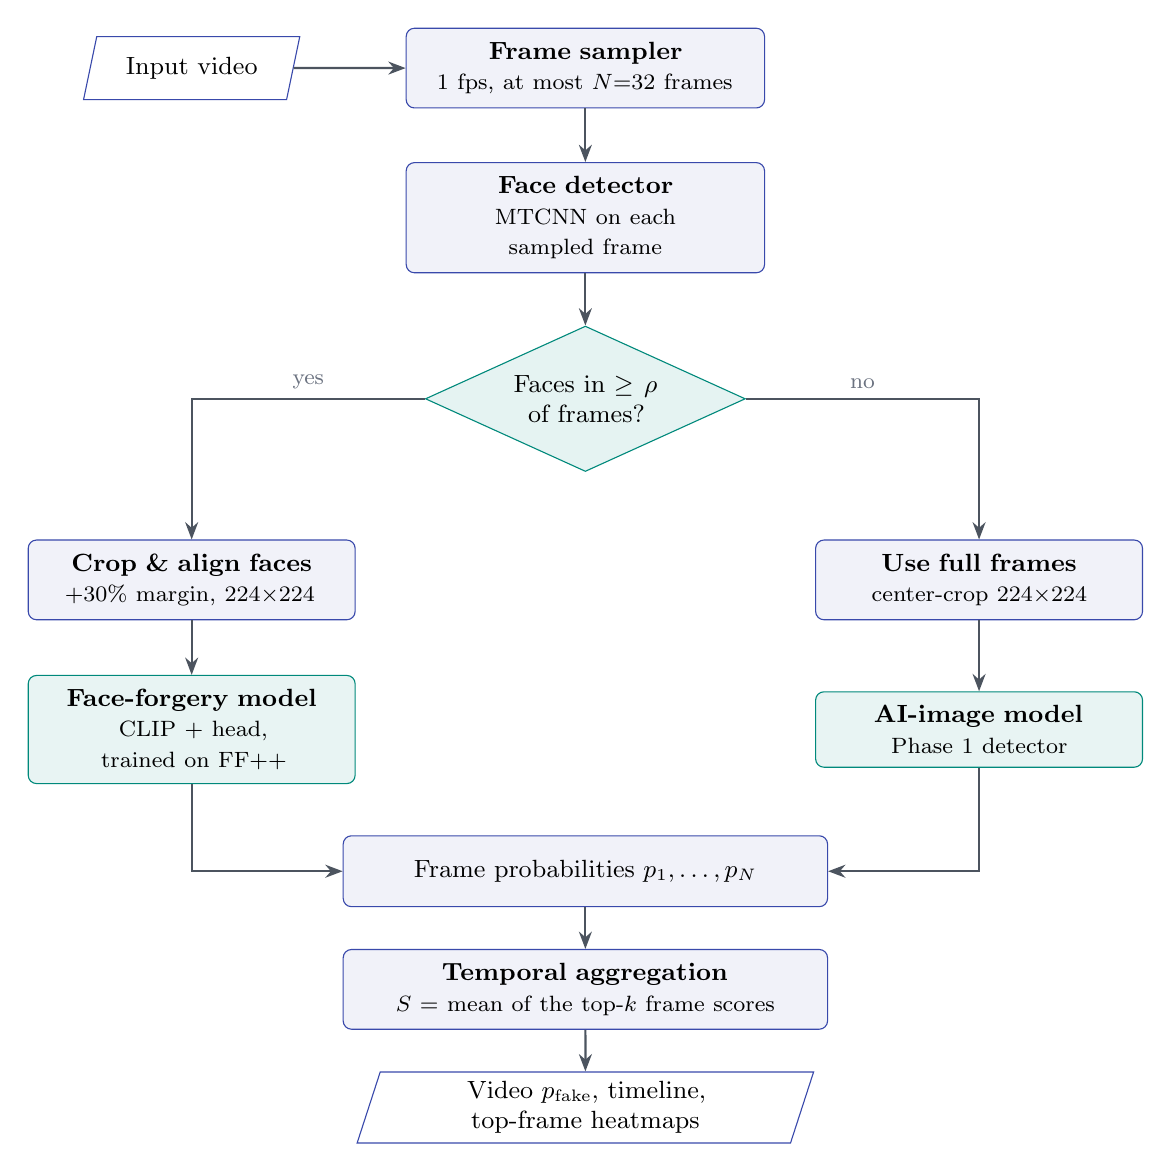
\begin{tikzpicture}
  \node[io, text width=2.2cm] (in) at (2.2,0) {Input video};
  \node[block, text width=4.2cm] (samp) at (7.2,0) {\textbf{Frame sampler}\\ {\footnotesize 1 fps, at most $N{=}32$ frames}};
  \node[block, text width=4.2cm] (det) at (7.2,-1.9) {\textbf{Face detector}\\ {\footnotesize MTCNN on each sampled frame}};
  \node[decision, text width=2.4cm] (face) at (7.2,-4.2) {Faces in $\ge\rho$ of frames?};
  \node[block, text width=3.8cm] (crop) at (2.2,-6.5) {\textbf{Crop \& align faces}\\ {\footnotesize +30\% margin, $224{\times}224$}};
  \node[block, text width=3.8cm] (full) at (12.2,-6.5) {\textbf{Use full frames}\\ {\footnotesize center-crop $224{\times}224$}};
  \node[ablock, text width=3.8cm] (fm) at (2.2,-8.4) {\textbf{Face-forgery model}\\ {\footnotesize CLIP + head, trained on FF++}};
  \node[ablock, text width=3.8cm] (im) at (12.2,-8.4) {\textbf{AI-image model}\\ {\footnotesize Phase 1 detector}};
  \node[block, text width=5.8cm] (pt) at (7.2,-10.2) {Frame probabilities $p_1,\dots,p_N$};
  \node[block, text width=5.8cm] (agg) at (7.2,-11.7) {\textbf{Temporal aggregation}\\ {\footnotesize $S$ = mean of the top-$k$ frame scores}};
  \node[io, text width=5.0cm] (out) at (7.2,-13.2) {Video $p_{\text{fake}}$, timeline, top-frame heatmaps};

  \draw[flow] (in) -- (samp);
  \draw[flow] (samp) -- (det);
  \draw[flow] (det) -- (face);
  \draw[flow] (face.west) -| node[lbl, pos=0.25, above]{yes} (crop.north);
  \draw[flow] (face.east) -| node[lbl, pos=0.25, above]{no} (full.north);
  \draw[flow] (crop) -- (fm);
  \draw[flow] (full) -- (im);
  \draw[flow] (fm.south) |- (pt.west);
  \draw[flow] (im.south) |- (pt.east);
  \draw[flow] (pt) -- (agg);
  \draw[flow] (agg) -- (out);
\end{tikzpicture}
\end{diagram}
\caption{Phase 2 video pipeline ($\rho=0.5$ by default).}
\label{fig:video-pipeline}
\end{figure}

\subsection{Frame sampling}
Neighbouring frames are almost identical, so we sample frames at a fixed rate (1 frame per
second) up to a maximum of $N=32$ frames. This keeps the processing time of a video close to that
of 32 images.

\subsection{Face detection with MTCNN}
MTCNN~\cite{mtcnn} is a cascade of three small CNNs:
\begin{enumerate}
  \item \textbf{P-Net} scans an image pyramid and proposes candidate face windows;
  \item \textbf{R-Net} rejects most false candidates and refines the boxes;
  \item \textbf{O-Net} outputs the final box and five facial landmarks (eyes, nose, mouth corners).
\end{enumerate}
Overlapping boxes are merged with non-maximum suppression. We keep the largest face, enlarge the
box by 30\% (so the blending boundary around the face is included, where face-swap artifacts
usually appear), align it using the eye landmarks and resize it to $224{\times}224$.

\subsection{Frame-level classifier}
The face-forgery model has the same structure as the Phase~1 model (frozen CLIP features and a
logistic head), trained on face crops from FaceForensics++~\cite{ffpp}. Training, validation and
test sets are split \textbf{by video}, never by frame; otherwise frames from the same video would
appear in both training and test data and the results would be falsely high.

\subsection{Temporal aggregation}
A manipulated video may look fake only in some frames, so a plain average can hide it. We compare
three ways of turning frame probabilities $p_1,\dots,p_N$ into one video score:
\begin{equation}
  S_{\text{mean}}=\frac{1}{N}\sum_{t=1}^{N}p_t,\qquad
  S_{\max}=\max_t p_t,\qquad
  S_{\text{top-}k}=\frac{1}{k}\sum_{t\in\mathcal{T}_k}p_t,\quad k=\lceil qN\rceil,
  \label{eq:agg}
\end{equation}
where $\mathcal{T}_k$ holds the $k$ frames with the highest scores and $q=0.2$. The top-$k$ mean
is our default: it reacts to short manipulated segments but is less noisy than the maximum. The
final choice is made on the validation set, and the video score is calibrated with
Equation~\ref{eq:platt}.

\subsection{Explanation}
The report shows (1) a \textbf{timeline} of $p_t$ over the video, so the user can see
\emph{when} the manipulation happens, and (2) Grad-CAM or patch heatmaps for the three frames with
the highest scores.

\begin{algorithm}[htbp]
\caption{Video inference}
\label{alg:video}
\begin{algorithmic}[1]
\Require video $V$, rate $r$, max frames $N$, face detector $\mathcal{F}$, face model $f_{\text{face}}$,
         image model $f_{\text{img}}$, face threshold $\rho$, top fraction $q$
\Ensure video probability $S$, frame timeline $\{p_t\}$, heatmaps
\State $\{I_1,\dots,I_N\}\gets\textsc{SampleFrames}(V,r,N)$
\For{$t=1$ to $N$}
  \State $B_t\gets\mathcal{F}(I_t)$ \Comment{face boxes and landmarks}
\EndFor
\If{$\lvert\{t: B_t\neq\emptyset\}\rvert\ \ge\ \rho N$} \Comment{face mode}
  \For{each $t$ with $B_t\neq\emptyset$}
    \State $p_t\gets f_{\text{face}}\bigl(\textsc{CropAlign}(I_t,\ \text{largest box in }B_t,\ 30\%)\bigr)$
  \EndFor
\Else \Comment{full-frame mode}
  \For{$t=1$ to $N$}
    \State $p_t\gets f_{\text{img}}\bigl(\textsc{CenterCrop}(I_t)\bigr)$
  \EndFor
\EndIf
\State $k\gets\lceil q\cdot(\text{number of scored frames})\rceil$;\quad $S\gets$ mean of the $k$ largest $p_t$
\State $S\gets\sigma(a\,\operatorname{logit}(S)+c)$ \Comment{calibration}
\State \Return $S$, $\{p_t\}$, heatmaps of the 3 highest-scoring frames
\end{algorithmic}
\end{algorithm}

% =====================================================================
\section{Phase 3: Document Authenticity Algorithms}
\label{sec:document}
% =====================================================================

\subsection{Pipeline}
Document forgeries are \emph{local}: a few words or numbers are changed and the rest of the page is
genuine. The goal is therefore \textbf{localization}: find the edited pixels, not only decide
real or fake. The document pipeline (Figure~\ref{fig:doc-pipeline}) combines three kinds of
evidence: a pixel-level forensic model, logic checks on the text, and checks on the PDF file
structure.

\begin{figure}[htbp]
\centering
\begin{diagram}
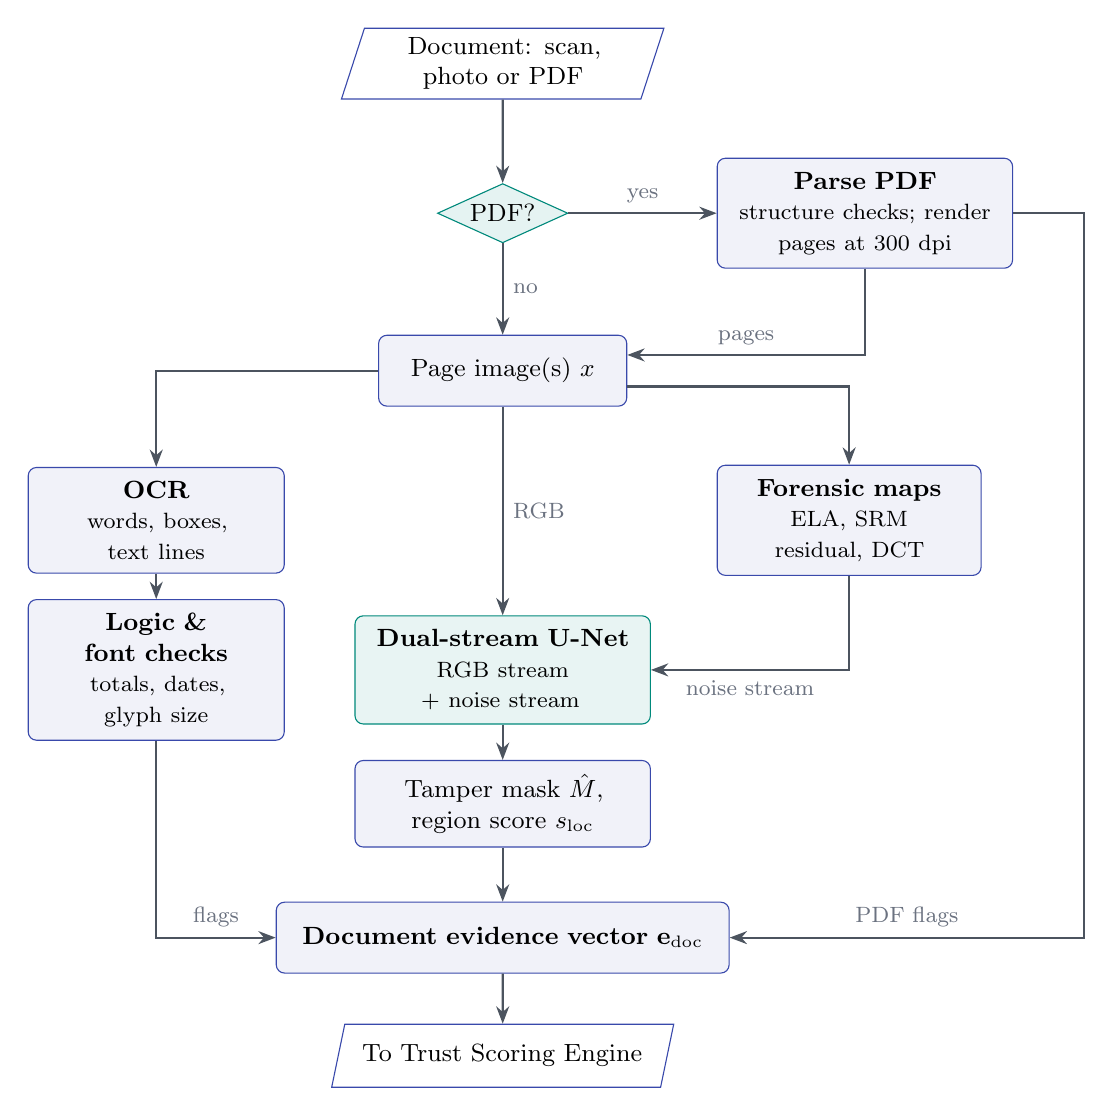
\begin{tikzpicture}
  \node[io, text width=3.3cm] (in) at (0,0) {Document: scan, photo or PDF};
  \node[decision] (pdf) at (0,-1.9) {PDF?};
  \node[block, text width=3.4cm] (parse) at (4.6,-1.9) {\textbf{Parse PDF}\\ {\footnotesize structure checks; render pages at 300 dpi}};
  \node[block, text width=2.8cm] (page) at (0,-3.9) {Page image(s) $x$};
  \node[block, text width=2.9cm] (ocr) at (-4.4,-5.8) {\textbf{OCR}\\ {\footnotesize words, boxes, text lines}};
  \node[block, text width=3.0cm] (maps) at (4.4,-5.8) {\textbf{Forensic maps}\\ {\footnotesize ELA, SRM residual, DCT}};
  \node[ablock, text width=3.4cm] (unet) at (0,-7.7) {\textbf{Dual-stream U-Net}\\ {\footnotesize RGB stream + noise stream}};
  \node[block, text width=2.9cm] (logic) at (-4.4,-7.7) {\textbf{Logic \& font checks}\\ {\footnotesize totals, dates, glyph size}};
  \node[block, text width=3.4cm] (mask) at (0,-9.4) {Tamper mask $\hat M$,\\ region score $s_{\text{loc}}$};
  \node[block, text width=5.4cm] (ev) at (0,-11.1) {\textbf{Document evidence vector} $\mathbf{e}_{\text{doc}}$};
  \node[io, text width=3.8cm] (out) at (0,-12.6) {To Trust Scoring Engine};

  \draw[flow] (in) -- (pdf);
  \draw[flow] (pdf) -- node[lbl, above]{yes} (parse);
  \draw[flow] (pdf) -- node[lbl, right]{no} (page);
  \draw[flow] (parse.south) |- node[lbl, pos=0.75, above]{pages} ([yshift=2mm]page.east);
  \draw[flow] ([yshift=-2mm]page.east) -| (maps.north);
  \draw[flow] (page.west) -| (ocr.north);
  \draw[flow] (page.south) -- node[lbl, right]{RGB} (unet.north);
  \draw[flow] (maps.south) |- node[lbl, pos=0.75, below]{noise stream} (unet.east);
  \draw[flow] (ocr) -- (logic);
  \draw[flow] (unet) -- (mask);
  \draw[flow] (mask) -- (ev);
  \draw[flow] (logic.south) |- node[lbl, pos=0.75, above]{flags} (ev.west);
  \draw[flow] (parse.east) -- ++(0.9,0) |- node[lbl, pos=0.75, above]{PDF flags} (ev.east);
  \draw[flow] (ev) -- (out);
\end{tikzpicture}
\end{diagram}
\caption{Phase 3 document pipeline.}
\label{fig:doc-pipeline}
\end{figure}

\subsection{Input handling and OCR}
PDFs are parsed twice: once for structure checks (Section~\ref{sec:pdfchecks}) and once rendered
to 300-dpi page images. Images are used directly. OCR (Tesseract~\cite{tesseract}, whose modern
versions use an LSTM line recognizer, or EasyOCR) returns every word with its bounding box. The
boxes are used by the logic checks, by the forgery generator (Algorithm~\ref{alg:forgery}) and to
snap the predicted mask to whole words in the report.

\subsection{Forensic maps}
\textbf{Error Level Analysis (ELA).} Re-saving a JPEG at a known quality changes regions that were
edited after the last save differently from untouched regions~\cite{ela}. With $J_q$ JPEG
compression at quality $q=90$:
\begin{equation}
  E(x)=\bigl\lvert x-J_q(x)\bigr\rvert .
  \label{eq:ela}
\end{equation}

\textbf{SRM noise residuals.} Spatial Rich Model filters from steganalysis~\cite{srm} remove image
content and keep local noise, where pasted or re-typed text looks different. We use the three
fixed kernels popularized for manipulation detection~\cite{rgbn}:
\begin{equation}
  \frac{1}{4}\!\begin{bmatrix}
  0&0&0&0&0\\ 0&-1&2&-1&0\\ 0&2&-4&2&0\\ 0&-1&2&-1&0\\ 0&0&0&0&0
  \end{bmatrix},\quad
  \frac{1}{12}\!\begin{bmatrix}
  -1&2&-2&2&-1\\ 2&-6&8&-6&2\\ -2&8&-12&8&-2\\ 2&-6&8&-6&2\\ -1&2&-2&2&-1
  \end{bmatrix},\quad
  \frac{1}{2}\!\begin{bmatrix}
  0&0&0&0&0\\ 0&0&0&0&0\\ 0&1&-2&1&0\\ 0&0&0&0&0\\ 0&0&0&0&0
  \end{bmatrix}.
  \label{eq:srm}
\end{equation}

\textbf{DCT coefficients.} JPEG stores each $8{\times}8$ block $f(x,y)$ as DCT coefficients
\begin{equation}
  F(u,v)=\tfrac14\,C(u)\,C(v)\sum_{x=0}^{7}\sum_{y=0}^{7} f(x,y)
  \cos\frac{(2x+1)u\pi}{16}\cos\frac{(2y+1)v\pi}{16},
  \label{eq:dct}
\end{equation}
with $C(0)=1/\sqrt2$ and $C(k)=1$ for $k>0$. The coefficients are then quantized, $Q(u,v)=\operatorname{round}\bigl(F(u,v)/q(u,v)\bigr)$. A pasted region
usually went through a different compression history, so its coefficient statistics do not
match the rest of the page. This is the main signal used by DocTamper~\cite{doctamper} and recent
document localization work~\cite{dhouib2026}. We feed clipped coefficient magnitudes of the
luminance channel as extra input channels.

\subsection{Dual-stream U-Net}
U-Net~\cite{unet} is an encoder--decoder network with skip connections that outputs a mask of the
same size as the input. Our \textbf{dual-stream} version (Figure~\ref{fig:unet}) has two encoders:
an RGB encoder (EfficientNet-B0, ImageNet weights) that sees the visible content, and a
lightweight noise encoder that sees the forensic maps $\mathbf{n}(x)=[\text{SRM};\text{ELA};\text{DCT}]$.
This follows the two-stream idea of RGB-N~\cite{rgbn}: edits that look natural in RGB often stand
out in the noise stream. At each decoder stage $l$, the up-sampled decoder features are
concatenated with the skip features of \emph{both} encoders:
\begin{equation}
  D_l=\operatorname{Conv}\bigl([\operatorname{Up}(D_{l+1});\,E^{r}_{l};\,E^{n}_{l}]\bigr),\qquad
  \hat M=\sigma\bigl(\operatorname{Conv}_{1\times1}(D_1)\bigr).
\end{equation}

\begin{figure}[htbp]
\centering
\begin{diagram}
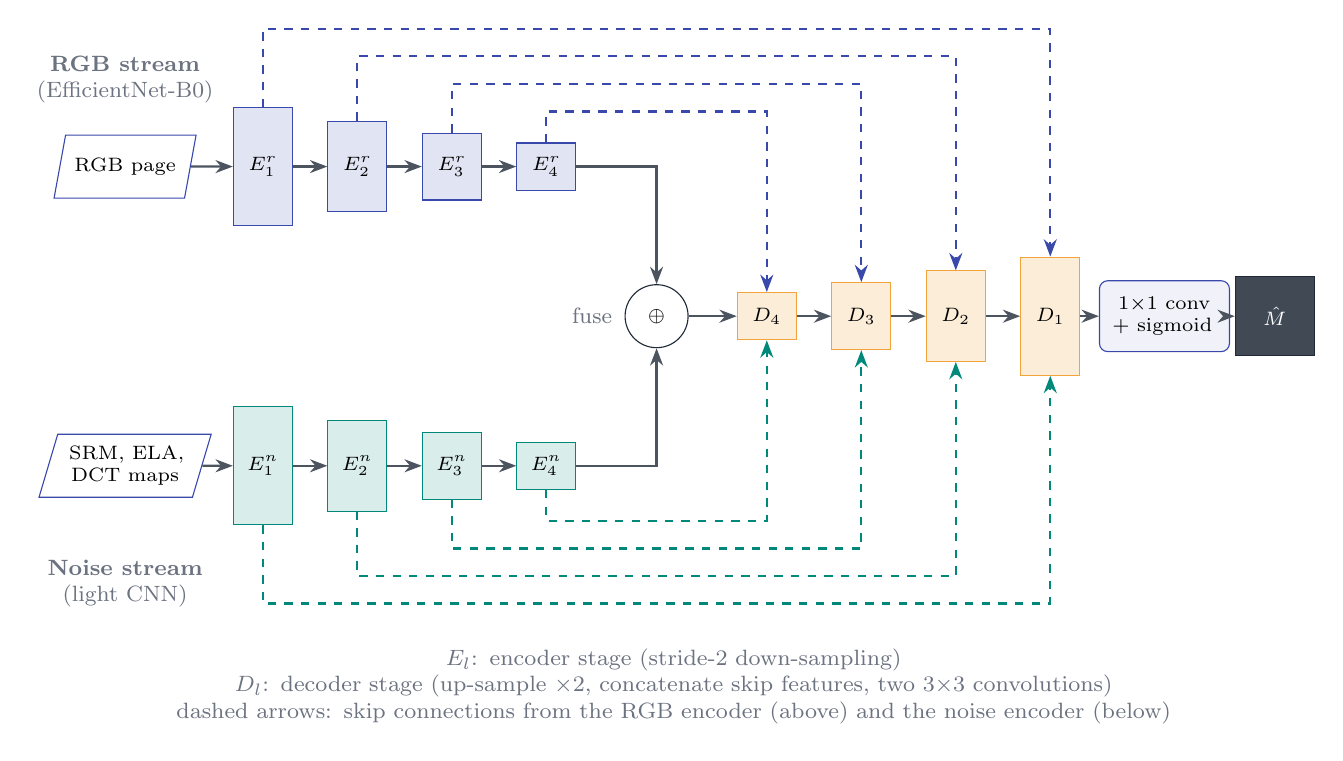
\begin{tikzpicture}[font=\scriptsize]
  % RGB encoder
  \node[draw=cPrimary, fill=cPrimary!15, minimum width=0.75cm, minimum height=1.5cm]  (r1) at (0,1.9)   {$E^{r}_1$};
  \node[draw=cPrimary, fill=cPrimary!15, minimum width=0.75cm, minimum height=1.15cm] (r2) at (1.2,1.9) {$E^{r}_2$};
  \node[draw=cPrimary, fill=cPrimary!15, minimum width=0.75cm, minimum height=0.85cm] (r3) at (2.4,1.9) {$E^{r}_3$};
  \node[draw=cPrimary, fill=cPrimary!15, minimum width=0.75cm, minimum height=0.6cm]  (r4) at (3.6,1.9) {$E^{r}_4$};
  % Noise encoder
  \node[draw=cAccent, fill=cAccent!15, minimum width=0.75cm, minimum height=1.5cm]  (n1) at (0,-1.9)   {$E^{n}_1$};
  \node[draw=cAccent, fill=cAccent!15, minimum width=0.75cm, minimum height=1.15cm] (n2) at (1.2,-1.9) {$E^{n}_2$};
  \node[draw=cAccent, fill=cAccent!15, minimum width=0.75cm, minimum height=0.85cm] (n3) at (2.4,-1.9) {$E^{n}_3$};
  \node[draw=cAccent, fill=cAccent!15, minimum width=0.75cm, minimum height=0.6cm]  (n4) at (3.6,-1.9) {$E^{n}_4$};
  % Bottleneck
  \node[circle, draw=cInk, fill=white, minimum size=0.8cm] (b) at (5.0,0) {$\oplus$};
  \node[lbl, left=1pt of b] {fuse};
  % Decoder
  \node[draw=cAmber, fill=cAmber!20, minimum width=0.75cm, minimum height=0.6cm]  (d4) at (6.4,0)  {$D_4$};
  \node[draw=cAmber, fill=cAmber!20, minimum width=0.75cm, minimum height=0.85cm] (d3) at (7.6,0)  {$D_3$};
  \node[draw=cAmber, fill=cAmber!20, minimum width=0.75cm, minimum height=1.15cm] (d2) at (8.8,0)  {$D_2$};
  \node[draw=cAmber, fill=cAmber!20, minimum width=0.75cm, minimum height=1.5cm]  (d1) at (10.0,0) {$D_1$};
  \node[block, font=\scriptsize, text width=1.3cm] (head) at (11.45,0) {$1{\times}1$ conv\\ + sigmoid};
  \node[draw=cInk, fill=cInk!85, text=white, minimum width=1.0cm, minimum height=1.0cm] (m) at (12.85,0) {$\hat M$};
  % Inputs
  \node[io, font=\scriptsize, text width=1.3cm] (xr) at (-1.75,1.9) {RGB page};
  \node[io, font=\scriptsize, text width=1.5cm] (xn) at (-1.75,-1.9) {SRM, ELA,\\ DCT maps};

  \draw[flow] (xr) -- (r1);  \draw[flow] (r1) -- (r2); \draw[flow] (r2) -- (r3); \draw[flow] (r3) -- (r4);
  \draw[flow] (xn) -- (n1);  \draw[flow] (n1) -- (n2); \draw[flow] (n2) -- (n3); \draw[flow] (n3) -- (n4);
  \draw[flow] (r4.east) -| (b.north);
  \draw[flow] (n4.east) -| (b.south);
  \draw[flow] (b) -- (d4); \draw[flow] (d4) -- (d3); \draw[flow] (d3) -- (d2); \draw[flow] (d2) -- (d1);
  \draw[flow] (d1) -- (head); \draw[flow] (head) -- (m);
  % Skip connections from the RGB encoder (above)
  \draw[dflow, draw=cPrimary] (r4.north) -- (r4.north |- 0,2.6)  -| (d4.north);
  \draw[dflow, draw=cPrimary] (r3.north) -- (r3.north |- 0,2.95) -| (d3.north);
  \draw[dflow, draw=cPrimary] (r2.north) -- (r2.north |- 0,3.3)  -| (d2.north);
  \draw[dflow, draw=cPrimary] (r1.north) -- (r1.north |- 0,3.65) -| (d1.north);
  % Skip connections from the noise encoder (below)
  \draw[dflow, draw=cAccent] (n4.south) -- (n4.south |- 0,-2.6)  -| (d4.south);
  \draw[dflow, draw=cAccent] (n3.south) -- (n3.south |- 0,-2.95) -| (d3.south);
  \draw[dflow, draw=cAccent] (n2.south) -- (n2.south |- 0,-3.3)  -| (d2.south);
  \draw[dflow, draw=cAccent] (n1.south) -- (n1.south |- 0,-3.65) -| (d1.south);
  % Labels
  \node[lbl] at (-1.75,3.0) {\textbf{RGB stream}\\(EfficientNet-B0)};
  \node[lbl] at (-1.75,-3.4) {\textbf{Noise stream}\\(light CNN)};
  \node[lbl, text width=15cm] at (5.2,-4.7) {$E_l$: encoder stage (stride-2 down-sampling)\\ $D_l$: decoder stage (up-sample $\times2$, concatenate skip features, two $3{\times}3$ convolutions)\\ dashed arrows: skip connections from the RGB encoder (above) and the noise encoder (below)};
\end{tikzpicture}
\end{diagram}
\caption{Dual-stream U-Net for tamper localization.}
\label{fig:unet}
\end{figure}

\textbf{Loss.} Edited pixels are usually less than 5\% of a page, so plain cross-entropy would
learn to predict ``nothing is edited''. We add the Dice loss~\cite{vnet}, which measures overlap
and is not dominated by the many untouched pixels:
\begin{equation}
  \mathcal{L}_{\text{Dice}}=1-\frac{2\sum_i\hat M_i M_i+\epsilon}{\sum_i\hat M_i+\sum_i M_i+\epsilon},
  \qquad
  \mathcal{L}_{\text{doc}}=\mathcal{L}_{\text{BCE}}+\mathcal{L}_{\text{Dice}} .
  \label{eq:dice}
\end{equation}
Pages are processed as overlapping $512{\times}512$ windows and the predictions are averaged.
The page-level \textbf{localization score} is the mean of the top 1\% pixel probabilities:
$s_{\text{loc}}=\operatorname{mean}\bigl(\text{top }1\%\text{ of }\hat M\bigr)$.

\subsection{Synthetic forgery generation}
Public document-forgery datasets need approval and are limited, so we generate our own training
data with exact ground-truth masks (Algorithm~\ref{alg:forgery}). Because models trained only on
synthetic forgeries often fail on real ones~\cite{rtm,dhouib2026}, we (1) apply realistic
after-effects such as JPEG re-saving and scanning noise, (2) include clean documents that went
through the same after-effects as negatives, so the model cannot use the after-effects as a
shortcut, and (3) always test on \emph{real} human-made forgeries (RTM~\cite{rtm}).

\begin{algorithm}[htbp]
\caption{Synthetic document forgery generation}
\label{alg:forgery}
\begin{algorithmic}[1]
\Require clean documents $\mathcal{C}$, OCR engine, operations $\mathcal{O}=\{\text{copy-move},\ \text{splice},\ \text{replace}\}$
\Ensure training pairs $\{(x',M)\}$ of images and masks
\For{each clean document $x\in\mathcal{C}$}
  \State $W\gets\textsc{OCR}(x)$ \Comment{word bounding boxes}
  \State $x'\gets x$;\quad $M\gets\mathbf{0}$ (same size as $x$)
  \State choose an operation $o\in\mathcal{O}$ and $m\in\{1,2,3\}$ target words at random
  \For{each target word box $w$}
    \If{$o=$ copy-move}
      \State copy another word or number region $u$ of $x$ into $w$
    \ElsIf{$o=$ splice}
      \State paste a region $u$ from another document $x_2\in\mathcal{C}$ into $w$
    \Else
      \State fill $w$ with local background and render new text in the closest font and size
    \EndIf
    \State $M[w]\gets1$
  \EndFor
  \State $(x',M)\gets\textsc{PostProcess}(x',M)$ \Comment{random JPEG 60--95, blur, noise, small rotation}
  \State save $(x',M)$ and the authentic pair $(\textsc{PostProcess}(x),\mathbf{0})$
\EndFor
\end{algorithmic}
\end{algorithm}

\subsection{Logic and consistency checks}
Some forgeries are pixel-perfect but \emph{logically} wrong. Recent text-forensics work combines
visual evidence with this kind of reasoning~\cite{logiclens}. Using the OCR output:
\begin{itemize}
  \item \textbf{Arithmetic check} (invoices, receipts): with quantities $q_i$, unit prices $u_i$ and
        printed total $T_{\text{total}}$, raise a flag if
        $\bigl\lvert\sum_i q_i u_i-T_{\text{total}}\bigr\rvert>\delta$ (for example $\delta=1$ currency unit).
  \item \textbf{Date check:} invalid dates, or an issue date after a due date.
  \item \textbf{Font consistency:} for each word $w$ with height $h_w$ on a text line, compute the
        modified z-score against the other words on that line and flag $\lvert M_w\rvert>3.5$:
        \begin{equation}
          M_w=\frac{0.6745\,\bigl(h_w-\operatorname{median}(h)\bigr)}{\operatorname{MAD}(h)} .
          \label{eq:modz}
        \end{equation}
        The same test is applied to the baseline position and character spacing.
\end{itemize}

\subsection{PDF structure checks}
\label{sec:pdfchecks}
Many real forgeries are edited PDFs, not scans. A PDF editor usually leaves traces in the file
itself~\cite{pdftamper}. Using PyMuPDF / pikepdf we check:
\begin{itemize}
  \item \textbf{incremental updates:} more than one \texttt{\%\%EOF} marker means content was appended after the first save;
  \item \textbf{dates:} modification date later than creation date;
  \item \textbf{producer:} creator and producer fields that name an editing tool;
  \item \textbf{fonts:} extra font subsets used for only a few characters on a page;
  \item \textbf{overlays:} white rectangles drawn on top of existing text.
\end{itemize}

\begin{algorithm}[htbp]
\caption{Document inference}
\label{alg:doc-infer}
\begin{algorithmic}[1]
\Require document $D$, U-Net $U$, OCR engine, rule checks
\Ensure localization score $s_{\text{loc}}$, masks $\{\hat M_j\}$, flags $\mathbf{f}$
\State $\mathbf{f}\gets\emptyset$
\If{$D$ is a PDF}
  \State $\mathbf{f}\gets\mathbf{f}\cup\textsc{PDFChecks}(D)$;\quad $\{x_j\}\gets\textsc{Render}(D,\ 300\text{ dpi})$
\Else
  \State $\{x_j\}\gets\{D\}$
\EndIf
\For{each page $x_j$}
  \State $\mathbf{n}_j\gets[\textsc{SRM}(x_j);\ \textsc{ELA}(x_j);\ \textsc{DCT}(x_j)]$
  \State $\hat M_j\gets U(x_j,\mathbf{n}_j)$ \Comment{overlapping $512{\times}512$ windows}
  \State $W_j\gets\textsc{OCR}(x_j)$;\quad $\mathbf{f}\gets\mathbf{f}\cup\textsc{LogicChecks}(W_j)\cup\textsc{FontChecks}(W_j)$
\EndFor
\State $s_{\text{loc}}\gets\max_j\ \operatorname{mean}\bigl(\text{top }1\%\text{ of }\hat M_j\bigr)$
\State \Return $s_{\text{loc}}$, $\{\hat M_j\}$, $\mathbf{f}$
\end{algorithmic}
\end{algorithm}

% =====================================================================
\section{Unified Trust Scoring Engine}
\label{sec:trust}
% =====================================================================

\subsection{Evidence fusion}
Each pipeline produces an evidence vector $\mathbf{e}\in\mathbb{R}^{d}$ (Figure~\ref{fig:trust}),
for example the model logit, the spectrum peak score, the localization score $s_{\text{loc}}$ and
binary rule flags. A logistic-regression fusion model, trained on the validation set of each
content type, turns it into a probability of manipulation:
\begin{equation}
  p_{\text{manip}}=\sigma\bigl(\boldsymbol{\beta}^{\top}\mathbf{e}+\beta_0\bigr).
  \label{eq:fusion}
\end{equation}
Logistic regression is chosen on purpose: its weights $\boldsymbol{\beta}$ show how much each piece
of evidence contributed, which feeds directly into the explanation.

\begin{figure}[htbp]
\centering
\begin{diagram}
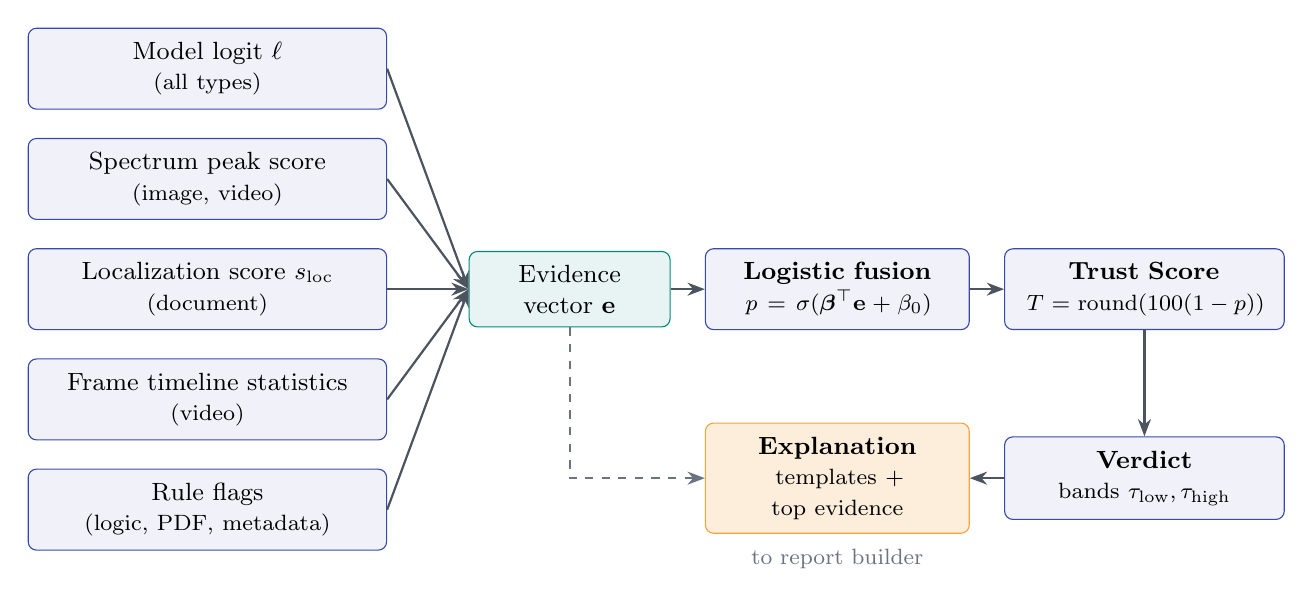
\begin{tikzpicture}
  \node[block, text width=4.2cm] (s1) at (0,2.8)  {Model logit $\ell$\\ {\footnotesize (all types)}};
  \node[block, text width=4.2cm] (s2) at (0,1.4)  {Spectrum peak score\\ {\footnotesize (image, video)}};
  \node[block, text width=4.2cm] (s3) at (0,0)    {Localization score $s_{\text{loc}}$\\ {\footnotesize (document)}};
  \node[block, text width=4.2cm] (s4) at (0,-1.4) {Frame timeline statistics\\ {\footnotesize (video)}};
  \node[block, text width=4.2cm] (s5) at (0,-2.8) {Rule flags\\ {\footnotesize (logic, PDF, metadata)}};
  \node[ablock, text width=2.2cm] (e) at (4.6,0) {Evidence vector $\mathbf{e}$};
  \node[block, text width=3.0cm] (fus) at (8.0,0) {\textbf{Logistic fusion}\\ {\footnotesize $p=\sigma(\boldsymbol\beta^\top\mathbf{e}+\beta_0)$}};
  \node[block, text width=3.2cm] (T) at (11.9,0) {\textbf{Trust Score}\\ {\footnotesize $T=\operatorname{round}(100(1-p))$}};
  \node[block, text width=3.2cm] (v) at (11.9,-2.4) {\textbf{Verdict}\\ {\footnotesize bands $\tau_{\text{low}},\tau_{\text{high}}$}};
  \node[vwarn, text width=3.0cm] (x) at (8.0,-2.4) {\textbf{Explanation}\\ {\footnotesize templates + top evidence}};
  \foreach \s in {s1,s2,s3,s4,s5} { \draw[flow] (\s.east) -- (e.west); }
  \draw[flow] (e) -- (fus);
  \draw[flow] (fus) -- (T);
  \draw[flow] (T) -- (v);
  \draw[flow] (v) -- (x);
  \draw[dflow] (e.south) |- (x.west);
  \node[lbl, below=2pt of x] {to report builder};
\end{tikzpicture}
\end{diagram}
\caption{Unified Trust Scoring Engine.}
\label{fig:trust}
\end{figure}

\subsection{Trust Score}
The Trust Score is the calibrated probability of authenticity on a 0--100 scale:
\begin{equation}
  T=\operatorname{round}\bigl(100\,(1-p_{\text{manip}})\bigr).
  \label{eq:trust}
\end{equation}
Because $p_{\text{manip}}$ is calibrated, $T=80$ means that, among validation files that received
a score near 80, about 80\% were authentic. The same meaning holds for images, videos and
documents, which is what makes one score across content types possible.

\subsection{Verdict bands and the human-review zone}
Detectors are often overconfident on inputs unlike their training data~\cite{calibdeepfake}.
Instead of forcing a real/fake decision, we use three bands (Figure~\ref{fig:bands}). The
thresholds are \emph{not} guessed: they are chosen on the validation set as the narrowest review
band for which the error rate of automatic decisions stays below a target $\alpha$
(Algorithm~\ref{alg:thresholds}). This is selective classification~\cite{selective}. A
possible upgrade is split conformal prediction~\cite{conformal}, which gives a formal
error guarantee when test data resembles the calibration data.

\begin{figure}[htbp]
\centering
\begin{diagram}
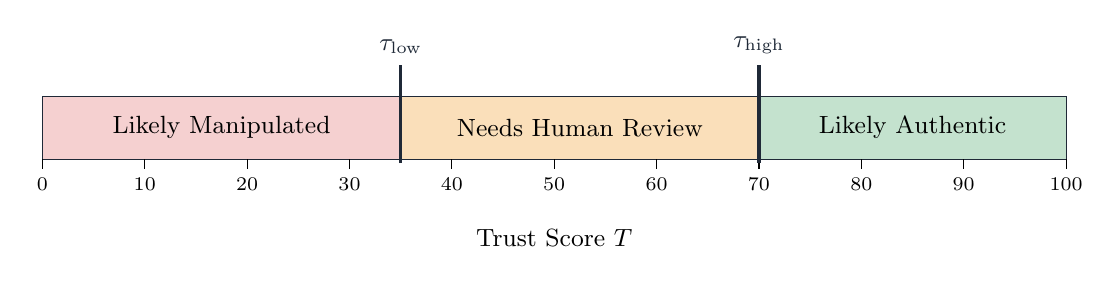
\begin{tikzpicture}[x=0.13cm]
  \fill[cRed!25]   (0,0)  rectangle (35,0.8);
  \fill[cAmber!35] (35,0) rectangle (70,0.8);
  \fill[cGreen!30] (70,0) rectangle (100,0.8);
  \draw[cInk] (0,0) rectangle (100,0.8);
  \node[font=\small] at (17.5,0.4) {Likely Manipulated};
  \node[font=\small] at (52.5,0.4) {Needs Human Review};
  \node[font=\small] at (85,0.4)   {Likely Authentic};
  \foreach \tk in {0,10,...,100} { \draw (\tk,0) -- (\tk,-0.12) node[below, font=\scriptsize] {\tk}; }
  \draw[very thick, cInk] (35,-0.05) -- (35,1.2) node[above, font=\small] {$\tau_{\text{low}}$};
  \draw[very thick, cInk] (70,-0.05) -- (70,1.2) node[above, font=\small] {$\tau_{\text{high}}$};
  \node[font=\small] at (50,-1.0) {Trust Score $T$};
\end{tikzpicture}
\end{diagram}
\caption{Verdict bands. The threshold values shown are only an illustration; real values come from Algorithm~\ref{alg:thresholds}.}
\label{fig:bands}
\end{figure}

\begin{algorithm}[htbp]
\caption{Choosing the verdict thresholds (selective classification)}
\label{alg:thresholds}
\begin{algorithmic}[1]
\Require validation scores and labels $\{(T_j,y_j)\}$ with $y_j=1$ for manipulated, target error $\alpha$ (e.g.\ 0.05)
\Ensure thresholds $\tau_{\text{low}}<\tau_{\text{high}}$
\State best $\gets$ none;\quad bestCoverage $\gets0$
\For{$\tau_{\text{low}}=0$ to $99$}
  \For{$\tau_{\text{high}}=\tau_{\text{low}}+1$ to $100$}
    \State $A\gets\{j:\ T_j\le\tau_{\text{low}}\ \text{or}\ T_j\ge\tau_{\text{high}}\}$ \Comment{decided automatically}
    \State err $\gets\frac{1}{\lvert A\rvert}\,\bigl\lvert\{j\in A:\ (T_j\le\tau_{\text{low}}\wedge y_j=0)\vee(T_j\ge\tau_{\text{high}}\wedge y_j=1)\}\bigr\rvert$
    \If{err $\le\alpha$ \textbf{and} $\lvert A\rvert>$ bestCoverage}
      \State best $\gets(\tau_{\text{low}},\tau_{\text{high}})$;\quad bestCoverage $\gets\lvert A\rvert$
    \EndIf
  \EndFor
\EndFor
\State \Return best
\end{algorithmic}
\end{algorithm}

\subsection{Explanation generation}
Explanations are built from templates filled with the evidence, never generated freely, so they
cannot claim something the system did not measure. The evidence items with the largest
contribution $\beta_i e_i$ are listed first.

\begin{table}[htbp]
\centering
\small
\begin{tabularx}{\linewidth}{@{}l Y@{}}
\toprule
\textbf{Evidence} & \textbf{Example sentence} \\
\midrule
High model score (image) & ``The image's visual features closely match AI-generated images.'' \\
High spectrum peak score & ``The frequency spectrum shows periodic peaks, a typical trace of AI up-sampling.'' \\
Frame timeline (video) & ``Frames between 0:06 and 0:09 show the strongest signs of face manipulation.'' \\
High $s_{\text{loc}}$ (document) & ``The highlighted amount has noise patterns that do not match the rest of the page.'' \\
Arithmetic flag & ``The line items add up to Rs.~42,500 but the printed total is Rs.~45,000.'' \\
PDF flag & ``The PDF was modified after it was created (2 incremental updates).'' \\
Review band & ``The evidence is mixed. A person should check this file before relying on it.'' \\
\bottomrule
\end{tabularx}
\caption{Explanation templates.}
\label{tab:templates}
\end{table}

% =====================================================================
\section{System Design Diagrams}
\label{sec:diagrams}
% =====================================================================

\subsection{Use case diagram}
The user uploads content and reads reports; the project team trains, calibrates and publishes models.
\begin{figure}[H]
\centering
\begin{diagram}
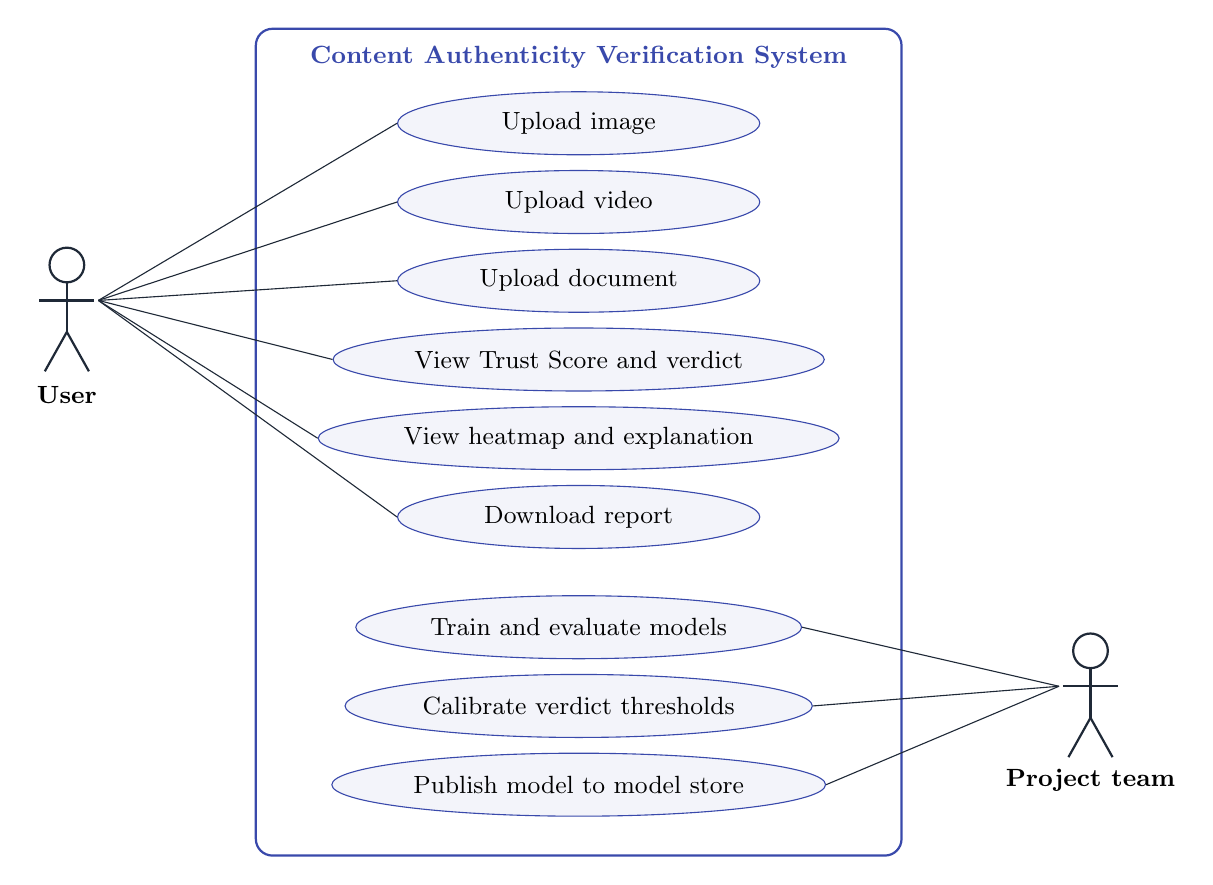
\begin{tikzpicture}
  \draw[cPrimary, thick, rounded corners=6pt] (2.4,1.0) rectangle (10.6,-9.5);
  \node[font=\small\bfseries, text=cPrimary, anchor=north] at (6.5,0.9) {Content Authenticity Verification System};
  \node[usecase] (u1) at (6.5,-0.2) {Upload image};
  \node[usecase] (u2) at (6.5,-1.2) {Upload video};
  \node[usecase] (u3) at (6.5,-2.2) {Upload document};
  \node[usecase] (u4) at (6.5,-3.2) {View Trust Score and verdict};
  \node[usecase] (u5) at (6.5,-4.2) {View heatmap and explanation};
  \node[usecase] (u6) at (6.5,-5.2) {Download report};
  \node[usecase] (u7) at (6.5,-6.6) {Train and evaluate models};
  \node[usecase] (u8) at (6.5,-7.6) {Calibrate verdict thresholds};
  \node[usecase] (u9) at (6.5,-8.6) {Publish model to model store};
  \pic at (0,-2.9) {actor};
  \node[font=\small\bfseries] at (0,-3.65) {User};
  \pic at (13,-7.8) {actor};
  \node[font=\small\bfseries] at (13,-8.55) {Project team};
  \foreach \u in {u1,u2,u3,u4,u5,u6} { \draw[cInk] (0.4,-2.45) -- (\u.west); }
  \foreach \u in {u7,u8,u9} { \draw[cInk] (12.6,-7.35) -- (\u.east); }
\end{tikzpicture}
\end{diagram}
\caption{Use case diagram.}
\label{fig:usecase}
\end{figure}

\subsection{Data flow diagrams}
Figure~\ref{fig:dfd0} shows the system as a single process; Figure~\ref{fig:dfd1} breaks it into its main processes and data stores.
\begin{figure}[H]
\centering
\begin{diagram}
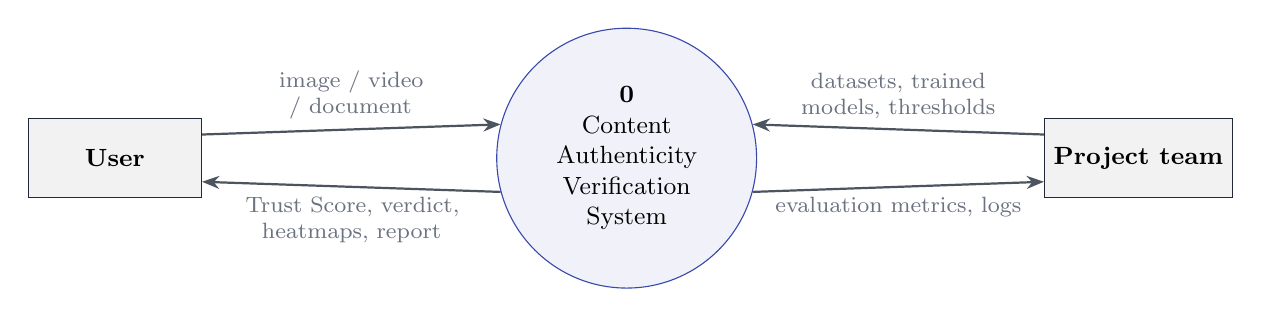
\begin{tikzpicture}
  \node[entity] (user) at (0,0) {User};
  \node[process, minimum size=3.3cm] (sys) at (6.5,0) {\textbf{0}\\ Content\\ Authenticity\\ Verification\\ System};
  \node[entity] (team) at (13,0) {Project team};
  \draw[flow] ([yshift=3mm]user.east) -- node[lbl, above, text width=3.2cm]{image / video / document} (sys.165);
  \draw[flow] (sys.195) -- node[lbl, below, text width=3.2cm]{Trust Score, verdict, heatmaps, report} ([yshift=-3mm]user.east);
  \draw[flow] ([yshift=3mm]team.west) -- node[lbl, above, text width=3.2cm]{datasets, trained models, thresholds} (sys.15);
  \draw[flow] (sys.345) -- node[lbl, below, text width=3.2cm]{evaluation metrics, logs} ([yshift=-3mm]team.west);
\end{tikzpicture}
\end{diagram}
\caption{DFD Level 0 (context diagram).}
\label{fig:dfd0}
\end{figure}

\begin{figure}[H]
\centering
\begin{diagram}
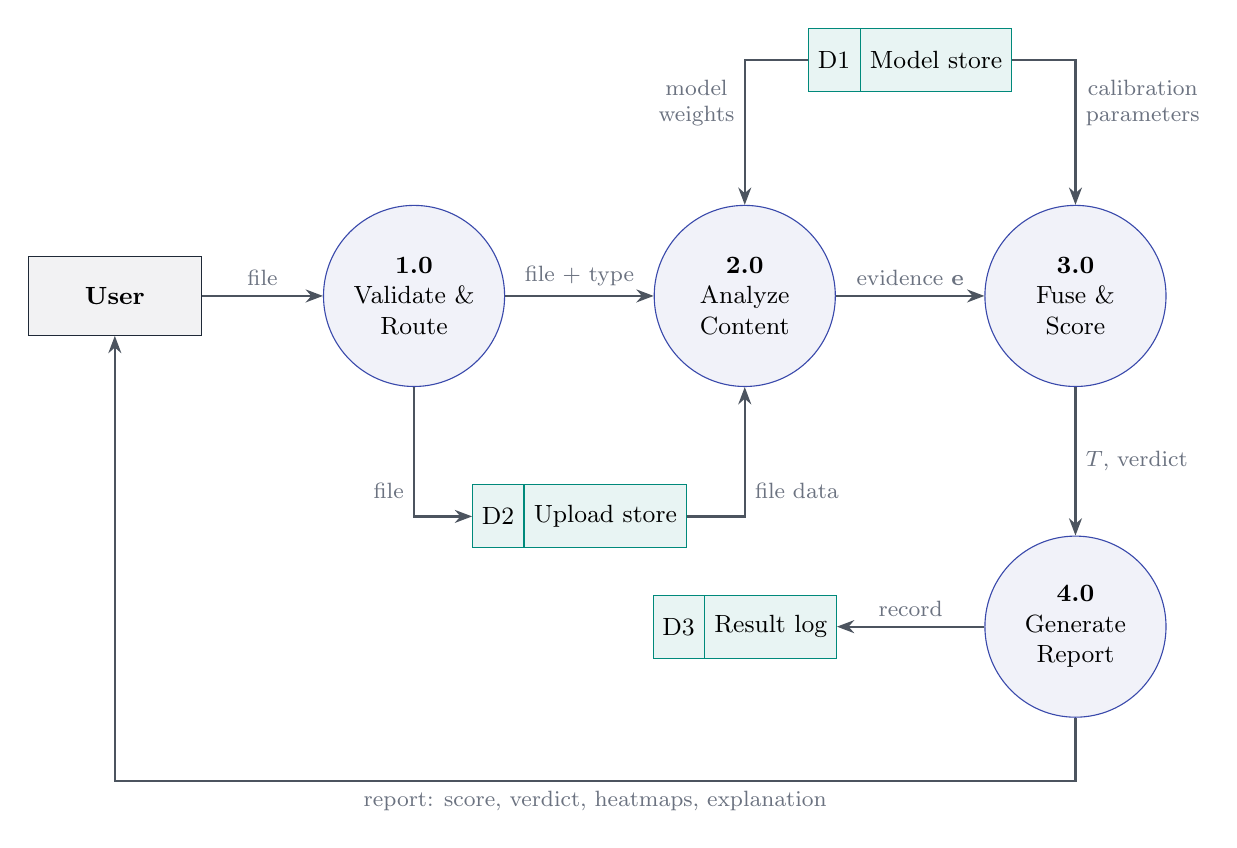
\begin{tikzpicture}
  \node[entity] (user) at (0,0) {User};
  \node[process] (p1) at (3.8,0)  {\textbf{1.0}\\ Validate \&\\ Route};
  \node[process] (p2) at (8.0,0)  {\textbf{2.0}\\ Analyze\\ Content};
  \node[process] (p3) at (12.2,0) {\textbf{3.0}\\ Fuse \&\\ Score};
  \node[process] (p4) at (12.2,-4.2) {\textbf{4.0}\\ Generate\\ Report};
  \node[datastore] (d2) at (5.9,-2.8) {D2 \nodepart{two} Upload store};
  \node[datastore] (d1) at (10.1,3.0) {D1 \nodepart{two} Model store};
  \node[datastore] (d3) at (8.0,-4.2) {D3 \nodepart{two} Result log};

  \draw[flow] (user) -- node[lbl, above]{file} (p1);
  \draw[flow] (p1) -- node[lbl, above]{file + type} (p2);
  \draw[flow] (p1.south) |- node[lbl, pos=0.4, left]{file} (d2.west);
  \draw[flow] (d2.east) -| node[lbl, pos=0.6, right]{file data} (p2.south);
  \draw[flow] (d1.west) -| node[lbl, pos=0.65, left]{model\\ weights} (p2.north);
  \draw[flow] (d1.east) -| node[lbl, pos=0.65, right]{calibration\\ parameters} (p3.north);
  \draw[flow] (p2) -- node[lbl, above]{evidence $\mathbf{e}$} (p3);
  \draw[flow] (p3) -- node[lbl, right]{$T$, verdict} (p4);
  \draw[flow] (p4) -- node[lbl, above]{record} (d3);
  \draw[flow] (p4.south) -- ++(0,-0.8) -| node[lbl, pos=0.25, below]{report: score, verdict, heatmaps, explanation} (user.south);
\end{tikzpicture}
\end{diagram}
\caption{DFD Level 1. Process 2.0 is expanded by the three pipeline flowcharts (Figures~\ref{fig:image-pipeline}, \ref{fig:video-pipeline} and~\ref{fig:doc-pipeline}).}
\label{fig:dfd1}
\end{figure}

\subsection{Sequence diagram}
The order of calls between components when a user analyzes one file.
\begin{figure}[H]
\centering
\begin{diagram}
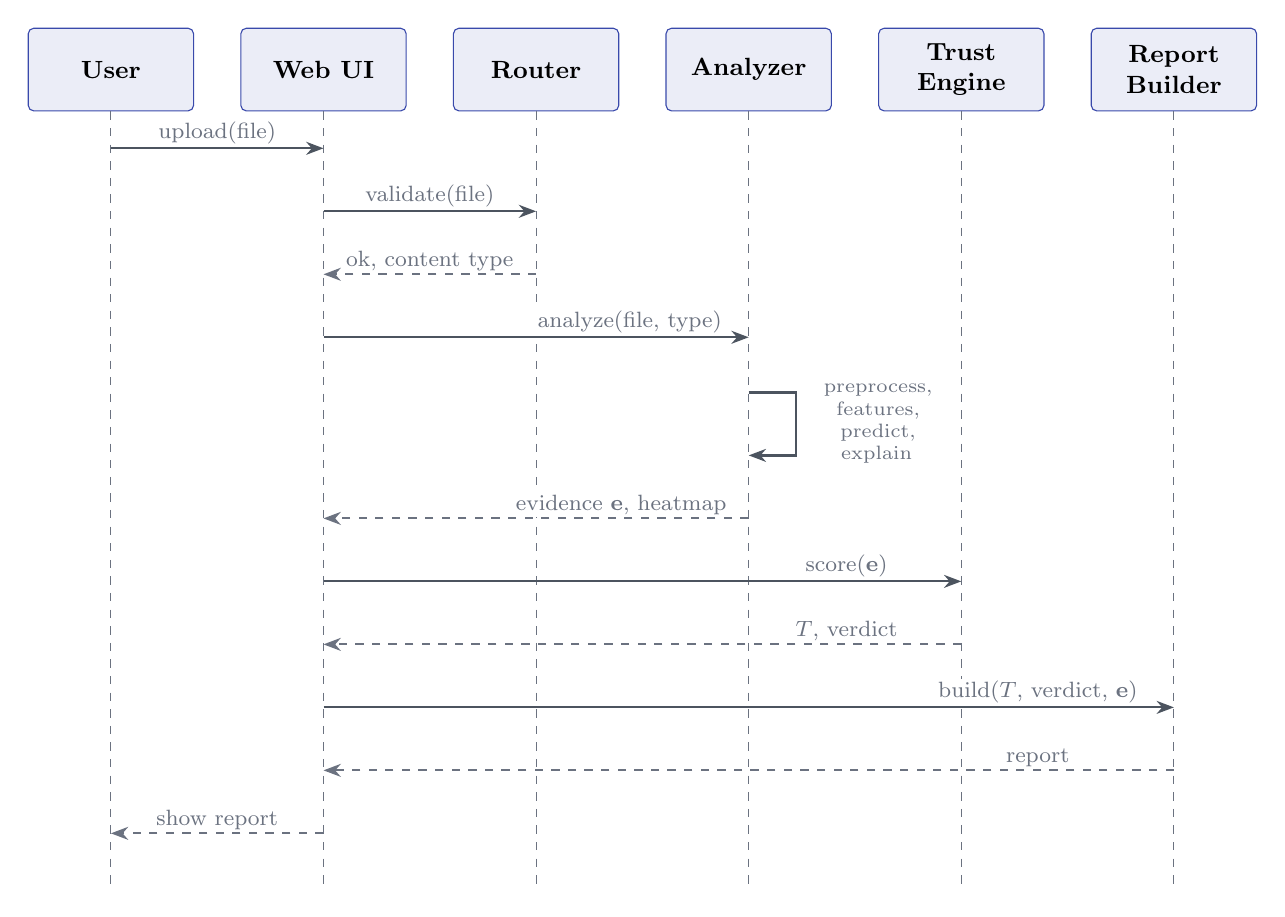
\begin{tikzpicture}
  \foreach \x/\n/\t in {0/U/User, 2.7/W/Web UI, 5.4/R/Router, 8.1/A/Analyzer, 10.8/T/{Trust\\ Engine}, 13.5/B/{Report\\ Builder}} {
    \node[seqhead, minimum height=1.05cm] (h\n) at (\x,0) {\t};
    \draw[dashed, cMuted] (h\n.south) -- (\x,-10.4);
  }
  \tikzset{msg/.style={lbl, above, fill=white, inner sep=1pt}}
  \draw[flow] (0,-1.0) -- node[msg]{upload(file)} (2.7,-1.0);
  \draw[flow] (2.7,-1.8) -- node[msg]{validate(file)} (5.4,-1.8);
  \draw[dflow] (5.4,-2.6) -- node[msg]{ok, content type} (2.7,-2.6);
  \draw[flow] (2.7,-3.4) -- node[msg, pos=0.72]{analyze(file, type)} (8.1,-3.4);
  \draw[flow] (8.1,-4.1) -- ++(0.6,0) -- ++(0,-0.8) -- ++(-0.6,0);
  \node[lbl, anchor=west, text width=1.7cm, font=\scriptsize] at (8.75,-4.5) {preprocess, features, predict, explain};
  \draw[dflow] (8.1,-5.7) -- node[msg, pos=0.3]{evidence $\mathbf{e}$, heatmap} (2.7,-5.7);
  \draw[flow] (2.7,-6.5) -- node[msg, pos=0.82]{score($\mathbf{e}$)} (10.8,-6.5);
  \draw[dflow] (10.8,-7.3) -- node[msg, pos=0.18]{$T$, verdict} (2.7,-7.3);
  \draw[flow] (2.7,-8.1) -- node[msg, pos=0.84]{build($T$, verdict, $\mathbf{e}$)} (13.5,-8.1);
  \draw[dflow] (13.5,-8.9) -- node[msg, pos=0.16]{report} (2.7,-8.9);
  \draw[dflow] (2.7,-9.7) -- node[msg]{show report} (0,-9.7);
\end{tikzpicture}
\end{diagram}
\caption{Sequence diagram for one analysis request (solid: call, dashed: return).}
\label{fig:sequence}
\end{figure}

\subsection{Class diagram}
The three analyzers share one abstract base class, and all of them return an \texttt{Evidence} object.
\begin{figure}[H]
\centering
\begin{diagram}
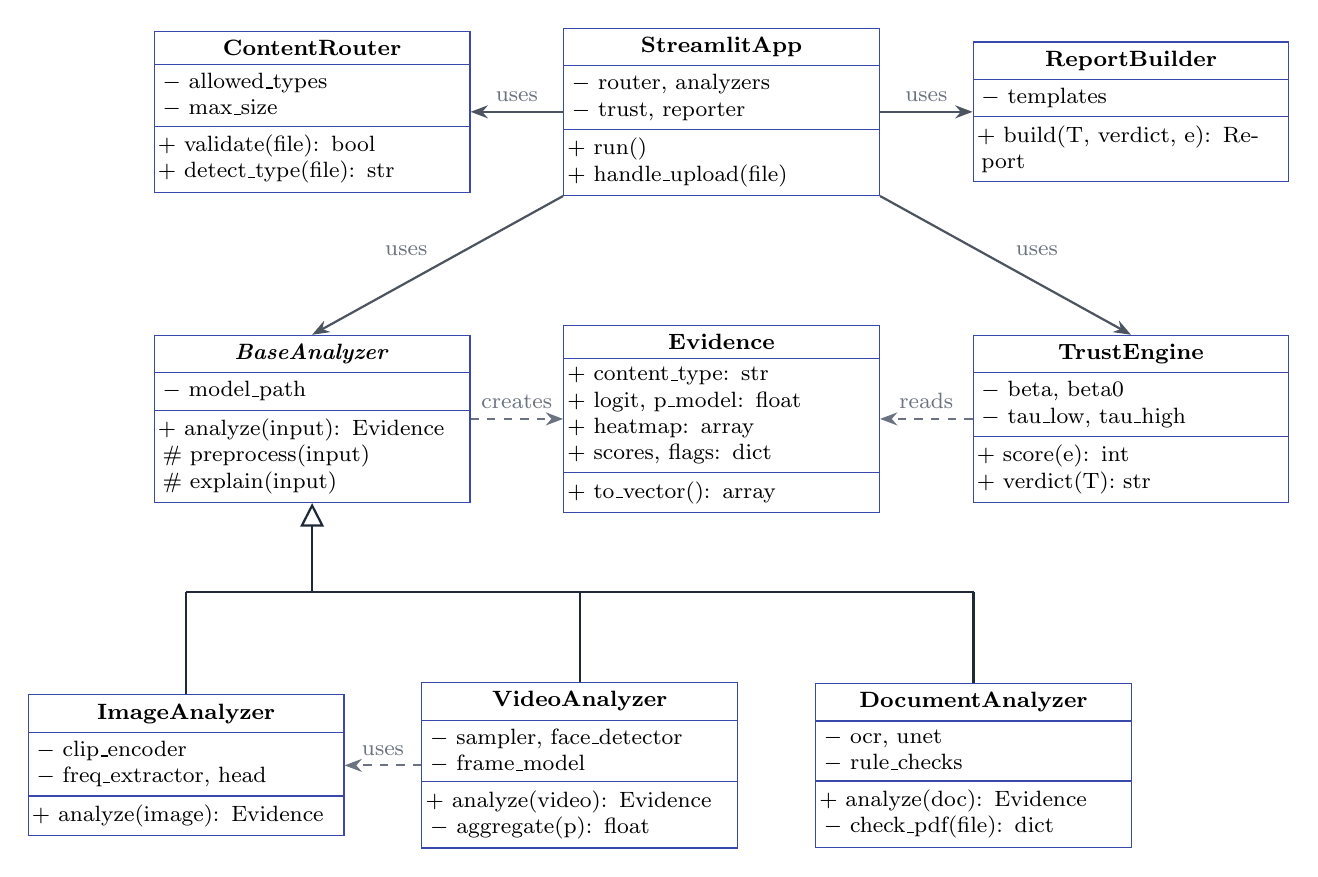
\begin{tikzpicture}
  \node[umlclass] (router) at (0,0) {\cname{ContentRouter}
    \nodepart{two} $-$ allowed\_types\\ $-$ max\_size
    \nodepart{three} $+$ validate(file): bool\\ $+$ detect\_type(file): str};
  \node[umlclass] (app) at (5.2,0) {\cname{StreamlitApp}
    \nodepart{two} $-$ router, analyzers\\ $-$ trust, reporter
    \nodepart{three} $+$ run()\\ $+$ handle\_upload(file)};
  \node[umlclass] (rep) at (10.4,0) {\cname{ReportBuilder}
    \nodepart{two} $-$ templates
    \nodepart{three} $+$ build(T, verdict, e): Report};
  \node[umlclass] (base) at (0,-3.9) {\cname{\textit{BaseAnalyzer}}
    \nodepart{two} $-$ model\_path
    \nodepart{three} $+$ analyze(input): Evidence\\ $\#$ preprocess(input)\\ $\#$ explain(input)};
  \node[umlclass] (ev) at (5.2,-3.9) {\cname{Evidence}
    \nodepart{two} $+$ content\_type: str\\ $+$ logit, p\_model: float\\ $+$ heatmap: array\\ $+$ scores, flags: dict
    \nodepart{three} $+$ to\_vector(): array};
  \node[umlclass] (trust) at (10.4,-3.9) {\cname{TrustEngine}
    \nodepart{two} $-$ beta, beta0\\ $-$ tau\_low, tau\_high
    \nodepart{three} $+$ score(e): int\\ $+$ verdict(T): str};
  \node[umlclass] (img) at (-1.6,-8.3) {\cname{ImageAnalyzer}
    \nodepart{two} $-$ clip\_encoder\\ $-$ freq\_extractor, head
    \nodepart{three} $+$ analyze(image): Evidence};
  \node[umlclass] (vid) at (3.4,-8.3) {\cname{VideoAnalyzer}
    \nodepart{two} $-$ sampler, face\_detector\\ $-$ frame\_model
    \nodepart{three} $+$ analyze(video): Evidence\\ $-$ aggregate(p): float};
  \node[umlclass] (doc) at (8.4,-8.3) {\cname{DocumentAnalyzer}
    \nodepart{two} $-$ ocr, unet\\ $-$ rule\_checks
    \nodepart{three} $+$ analyze(doc): Evidence\\ $-$ check\_pdf(file): dict};

  \draw[flow] (app.west) -- node[lbl, above]{uses} (router.east);
  \draw[flow] (app.east) -- node[lbl, above]{uses} (rep.west);
  \draw[flow] (app.south west) -- node[lbl, above left]{uses} (base.north);
  \draw[flow] (app.south east) -- node[lbl, above right]{uses} (trust.north);
  \draw[dflow] (base.east) -- node[lbl, above]{creates} (ev.west);
  \draw[dflow] (trust.west) -- node[lbl, above]{reads} (ev.east);
  \draw[thick, cInk] (img.north) -- (img.north |- 0,-6.1);
  \draw[thick, cInk] (vid.north) -- (vid.north |- 0,-6.1);
  \draw[thick, cInk] (doc.north) -- (doc.north |- 0,-6.1);
  \draw[thick, cInk] (img.north |- 0,-6.1) -- (doc.north |- 0,-6.1);
  \draw[thick, cInk, -{Triangle[open, length=3mm, width=3mm]}] (base.south |- 0,-6.1) -- (base.south);
  \draw[dflow] (vid.west) -- node[lbl, above]{uses} (img.east);
\end{tikzpicture}
\end{diagram}
\caption{Class diagram of the main software components.}
\label{fig:class}
\end{figure}

\subsection{Training and inference workflow}
Training runs offline on free GPUs; the web app only loads the exported files.
\begin{figure}[H]
\centering
\begin{diagram}
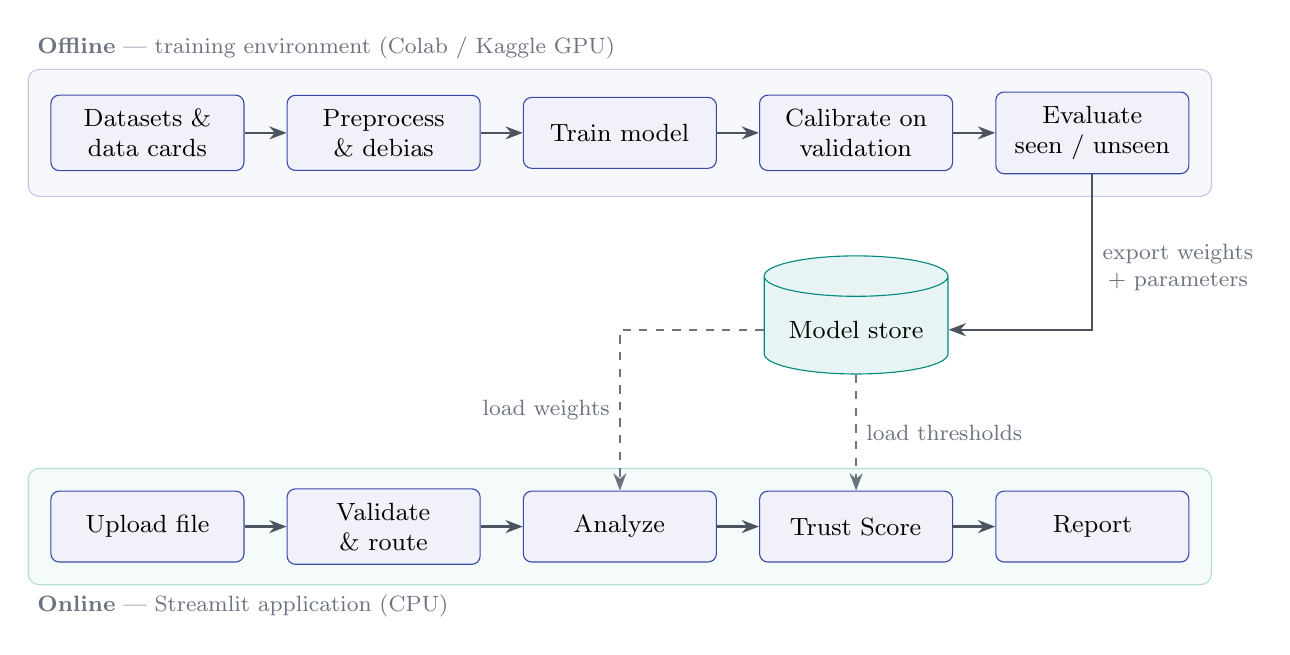
\begin{tikzpicture}
  \node[block, text width=2.1cm] (ds)  at (0,0)    {Datasets \&\\ data cards};
  \node[block, text width=2.1cm] (pp)  at (3.0,0)  {Preprocess \& debias};
  \node[block, text width=2.1cm] (tr)  at (6.0,0)  {Train model};
  \node[block, text width=2.1cm] (cb)  at (9.0,0)  {Calibrate on validation};
  \node[block, text width=2.1cm] (evl) at (12.0,0) {Evaluate seen / unseen};
  \node[store, text width=2.1cm] (ms)  at (9.0,-2.5) {Model store};
  \node[block, text width=2.1cm] (up)  at (0,-5.0)  {Upload file};
  \node[block, text width=2.1cm] (rt)  at (3.0,-5.0) {Validate \& route};
  \node[block, text width=2.1cm] (an)  at (6.0,-5.0) {Analyze};
  \node[block, text width=2.1cm] (ts)  at (9.0,-5.0) {Trust Score};
  \node[block, text width=2.1cm] (rp)  at (12.0,-5.0) {Report};

  \draw[flow] (ds) -- (pp); \draw[flow] (pp) -- (tr); \draw[flow] (tr) -- (cb); \draw[flow] (cb) -- (evl);
  \draw[flow] (evl.south) |- node[lbl, pos=0.3, right]{export weights\\ + parameters} (ms.east);
  \draw[flow] (up) -- (rt); \draw[flow] (rt) -- (an); \draw[flow] (an) -- (ts); \draw[flow] (ts) -- (rp);
  \draw[dflow] (ms.west) -| node[lbl, pos=0.75, left]{load weights} (an.north);
  \draw[dflow] (ms.south) -- node[lbl, right]{load thresholds} (ts.north);

  \begin{scope}[on background layer]
    \node[fit=(ds)(evl), fill=cPrimary!4, draw=cPrimary!30, rounded corners, inner sep=8pt,
          label={[lbl, anchor=south west]north west:{\textbf{Offline} --- training environment (Colab / Kaggle GPU)}}] {};
    \node[fit=(up)(rp), fill=cAccent!4, draw=cAccent!30, rounded corners, inner sep=8pt,
          label={[lbl, anchor=north west]south west:{\textbf{Online} --- Streamlit application (CPU)}}] {};
  \end{scope}
\end{tikzpicture}
\end{diagram}
\caption{Offline training and online inference share only the model store.}
\label{fig:workflow}
\end{figure}

\subsection{Deployment diagram}
Where each part of the system runs.
\begin{figure}[H]
\centering
\begin{diagram}
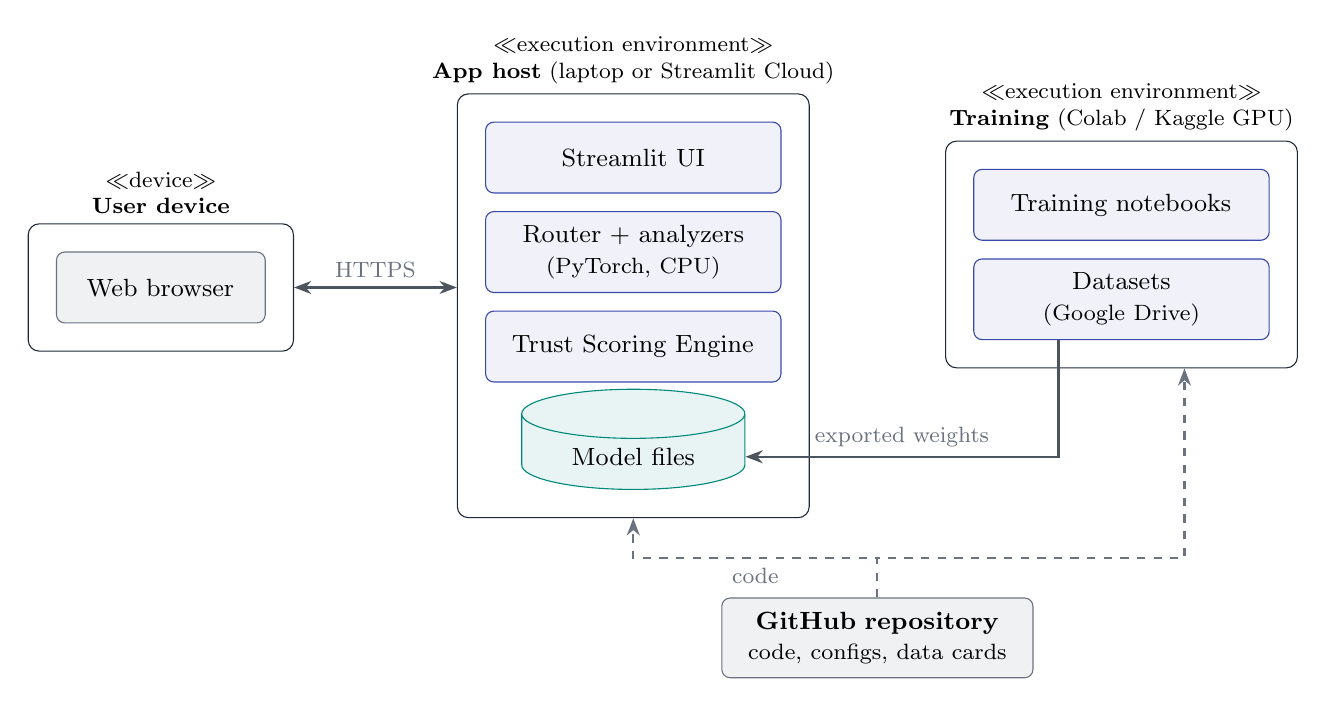
\begin{tikzpicture}
  % User device
  \node[gblock, text width=2.3cm] (br) at (0,-0.45) {Web browser};
  % App host
  \node[block, text width=3.4cm] (c1) at (6.0,1.2)  {Streamlit UI};
  \node[block, text width=3.4cm] (c2) at (6.0,0.0)  {Router + analyzers\\ {\footnotesize (PyTorch, CPU)}};
  \node[block, text width=3.4cm] (c3) at (6.0,-1.2) {Trust Scoring Engine};
  \node[store, text width=2.6cm, minimum height=1.2cm] (c4) at (6.0,-2.6) {Model files};
  % Training
  \node[block, text width=3.4cm] (t1) at (12.2,0.6)  {Training notebooks};
  \node[block, text width=3.4cm] (t2) at (12.2,-0.6) {Datasets\\ {\footnotesize (Google Drive)}};
  % Repo
  \node[gblock, text width=3.6cm] (repo) at (9.1,-4.9) {\textbf{GitHub repository}\\ {\footnotesize code, configs, data cards}};

  \node[fit=(br), draw=cInk, rounded corners, inner sep=10pt,
        label={[font=\footnotesize, align=center]above:{$\ll$device$\gg$\\ \textbf{User device}}}] (dev) {};
  \node[fit=(c1)(c2)(c3)(c4), draw=cInk, rounded corners, inner sep=10pt,
        label={[font=\footnotesize, align=center]above:{$\ll$execution environment$\gg$\\ \textbf{App host} (laptop or Streamlit Cloud)}}] (host) {};
  \node[fit=(t1)(t2), draw=cInk, rounded corners, inner sep=10pt,
        label={[font=\footnotesize, align=center]above:{$\ll$execution environment$\gg$\\ \textbf{Training} (Colab / Kaggle GPU)}}] (trn) {};

  \draw[<->, thick, cInk!80] (dev.east) -- node[lbl, above]{HTTPS} (dev.east -| host.west);
  \draw[flow] ([xshift=-0.8cm]t2.south) |- node[lbl, pos=0.75, above]{exported weights} (c4.east);
  \draw[dflow] (repo.north) -- ++(0,0.5) -| node[lbl, pos=0.25, below]{code} (host.south);
  \draw[dflow] (repo.north) -- ++(0,0.5) -| ([xshift=0.8cm]trn.south);
\end{tikzpicture}
\end{diagram}
\caption{Deployment diagram.}
\label{fig:deploy}
\end{figure}

% =====================================================================
\section{Data Design}
\label{sec:data}
% =====================================================================

\subsection{Datasets and splits}
\begin{table}[htbp]
\centering
\small
\begin{tabularx}{\linewidth}{@{}l l Y Y@{}}
\toprule
\textbf{Dataset} & \textbf{Phase} & \textbf{Use} & \textbf{Split rule} \\
\midrule
GenImage~\cite{genimage} (subsets) & 1 & Train on real + SD v1.4; test on 7 other generators & Official train/val split; start with about 10k real + 10k fake \\
Own 2026 test set & 1 & Unseen recent generators (SDXL / SD 3.5 class), prompts from COCO captions & Test only; real side = matching COCO photos \\
FaceForensics++~\cite{ffpp} (c23) & 2 & Train and seen test (4 manipulation methods) & By video ID \\
Celeb-DF v2~\cite{celebdf} & 2 & Unseen test & Test only \\
Clean documents + own forgeries & 3 & Train localization model & By source document \\
RTM~\cite{rtm} & 3 & Real human-made forgeries (unseen test) & Test only \\
DocTamper~\cite{doctamper}, OSTF~\cite{ostf} & 3 & Extra tests, if access is granted & Official splits \\
\bottomrule
\end{tabularx}
\caption{Datasets. Access for FaceForensics++, Celeb-DF and DocTamper must be requested from the authors.}
\label{tab:datasets}
\end{table}

\subsection{The Evidence object}
\label{sec:evidence-object}
Every pipeline returns the same structure, so the rest of the system never needs to know which
pipeline produced it.

{\small
\begin{verbatim}
@dataclass
class Evidence:
    content_type: str             # "image" | "video" | "document"
    logit: float                  # raw model score used by the fusion layer
    p_model: float                # calibrated probability of manipulation
    heatmap: np.ndarray | None    # H x W map in [0, 1]
    scores: dict[str, float]      # e.g. {"spectrum_peak": 3.1, "s_loc": 0.82}
    flags: dict[str, bool]        # e.g. {"total_mismatch": True}
    details: dict[str, Any]       # frame timeline, OCR boxes, text for the report

    def to_vector(self) -> np.ndarray: ...
\end{verbatim}
}

\subsection{Repository structure}
{\small
\begin{verbatim}
deepfake-detection/
  app/          Streamlit app: UI, router, report builder
  core/         Evidence, TrustEngine, shared utilities
  image/        Phase 1: preprocessing, CLIP and frequency features, training
  video/        Phase 2: frame sampling, face detection, aggregation
  document/     Phase 3: OCR, forensic maps, U-Net, rule checks, forgery generator
  eval/         evaluate.py, robustness tests, calibration plots
  notebooks/    Colab / Kaggle training notebooks
  models/       exported weights and calibration files (not stored in git)
  data/         data cards and split lists (images not stored in git)
  docs/         this document, project roadmap
  requirements.txt
\end{verbatim}
}

\subsection{Initial hyperparameters}
These are starting values; all are tuned on the validation set.

\begin{table}[htbp]
\centering
\small
\begin{tabularx}{\linewidth}{@{}l Y@{}}
\toprule
\textbf{Component} & \textbf{Setting} \\
\midrule
Image head & CLIP ViT-L/14 at $224{\times}224$; $K=64$ radial bins; logistic regression, $\lambda$ from $\{10^{-3},10^{-2},10^{-1}\}$ \\
EfficientNet-B0 baseline & AdamW, learning rate $10^{-4}$, batch 32, up to 10 epochs, early stopping on validation AUC \\
Augmentation & random JPEG quality 60--100 ($p=0.5$), random crop, horizontal flip \\
Video & 1 fps, $N\le32$ frames, face margin 30\%, $\rho=0.5$, top fraction $q=0.2$ \\
Document U-Net & $512{\times}512$ windows, EfficientNet-B0 encoder, AdamW $10^{-4}$, batch 8, 30 epochs, loss BCE + Dice, ELA quality 90 \\
Trust engine & target error of automatic decisions $\alpha=0.05$ \\
\bottomrule
\end{tabularx}
\caption{Initial hyperparameters.}
\label{tab:hparams}
\end{table}

% =====================================================================
\section{Evaluation Design}
\label{sec:evaluation}
% =====================================================================

\subsection{Protocols}
\begin{table}[H]
\centering
\small
\begin{tabularx}{\linewidth}{@{}l Y Y Y@{}}
\toprule
\textbf{Phase} & \textbf{Trained on} & \textbf{Unseen test} & \textbf{Main metrics} \\
\midrule
Image & Real + SD v1.4 (GenImage) & 7 other GenImage generators + own 2026 set & AUC and accuracy per generator, unseen average \\
Video & FaceForensics++ & Celeb-DF v2 & Frame-level and video-level AUC \\
Document & Own synthetic forgeries & RTM real forgeries (+ DocTamper, OSTF) & Pixel F1, IoU, image-level AUC \\
All & --- & JPEG 90/70/50, resize $\times0.5$, blur, screenshot & Robustness curves, ECE, review rate \\
\bottomrule
\end{tabularx}
\caption{Evaluation protocols. Seen and unseen results are always reported side by side.}
\label{tab:protocols}
\end{table}

\subsection{Metrics}
With TP, TN, FP, FN the true/false positives/negatives (``positive'' = manipulated):
\begin{equation}
\begin{aligned}
  \text{Accuracy}&=\frac{TP+TN}{TP+TN+FP+FN}, &\qquad \text{Precision}\ P&=\frac{TP}{TP+FP},\\[4pt]
  \text{Recall}\ R&=\frac{TP}{TP+FN}, &\qquad F_1&=\frac{2\,PR}{P+R}.
\end{aligned}
\end{equation}
\textbf{AUC} is the probability that a randomly chosen fake gets a higher score than a randomly
chosen real sample. It does not depend on a threshold, which matters because the best threshold
often shifts on unseen generators:
\begin{equation}
  \text{AUC}=\Pr\bigl(s(x^{+})>s(x^{-})\bigr).
\end{equation}
For localization, with predicted mask $\hat M$ (thresholded at 0.5) and true mask $M$:
\begin{equation}
  \text{IoU}=\frac{\lvert\hat M\cap M\rvert}{\lvert\hat M\cup M\rvert},\qquad
  F_1^{\text{pixel}}=\frac{2\,\lvert\hat M\cap M\rvert}{\lvert\hat M\rvert+\lvert M\rvert}.
\end{equation}
Calibration is measured with ECE (Equation~\ref{eq:ece}), and the review band with the share of
files sent to human review at the chosen error target.

% =====================================================================
\section{Non-Functional Requirements}
\label{sec:nfr}
% =====================================================================

\begin{table}[htbp]
\centering
\small
\begin{tabularx}{\linewidth}{@{}l Y@{}}
\toprule
\textbf{Requirement} & \textbf{Target} \\
\midrule
Performance & Image: result in under 5\,s on a laptop CPU. Video (30\,s clip): under 60\,s. Document: under 15\,s per page. \\
Supported inputs & Images: JPG, PNG, WEBP, BMP, TIFF, HEIC (up to 20\,MB). Videos: MP4, MOV, AVI, MKV, WEBM (up to 100\,MB, 2 minutes). Animated GIF/WEBP are treated as short videos. Documents: PDF (up to 10 pages), JPG, PNG, TIFF. Every file is identified by its signature bytes and converted to a standard internal form (RGB pixels, sampled frames or 300-dpi pages). \\
Reliability & Calibrated scores; uncertain cases go to the review band; no verdict without evidence. \\
Privacy & Uploads are processed in temporary storage and deleted at the end of the session; uploads are never used for training. \\
Usability & Colour-coded verdict, plain-language explanation, downloadable report. \\
Maintainability & Independent analyzers behind one \texttt{Evidence} interface; settings in configuration files; pinned package versions. \\
Reproducibility & Fixed random seeds, saved split lists, data cards and an experiment log. \\
Ethics & Datasets used under their research licences; the system supports human judgement and does not certify documents legally. \\
\bottomrule
\end{tabularx}
\caption{Non-functional requirements.}
\label{tab:nfr}
\end{table}

% =====================================================================
\section{Technology Stack}
\label{sec:stack}
% =====================================================================

\begin{table}[htbp]
\centering
\small
\begin{tabularx}{\linewidth}{@{}l Y@{}}
\toprule
\textbf{Purpose} & \textbf{Tools} \\
\midrule
Language and deep learning & Python 3.10+, PyTorch, \texttt{open\_clip} / Hugging Face \texttt{transformers}, \texttt{timm} \\
Classical ML and metrics & scikit-learn (logistic regression, calibration, AUC, ECE) \\
Image and signal processing & OpenCV, NumPy, SciPy, scikit-image (FFT, median filter, DCT, ELA) \\
Video & OpenCV (frame sampling), \texttt{facenet-pytorch} (MTCNN) \\
Documents & Tesseract / EasyOCR, \texttt{segmentation\_models\_pytorch} (U-Net), PyMuPDF, pikepdf \\
Explainability & \texttt{pytorch-grad-cam}, Matplotlib \\
Application & Streamlit \\
Training infrastructure & Google Colab, Kaggle (free GPU tiers), Google Drive \\
Collaboration & GitHub \\
\bottomrule
\end{tabularx}
\caption{Technology stack.}
\label{tab:stack}
\end{table}

% =====================================================================
\section{Implementation Timeline}
\label{sec:timeline}
% =====================================================================
Week~1 starts on 28 September 2026. Week-by-week tasks are in \texttt{PROJECT\_ROADMAP.md}.

\begin{figure}[htbp]
\centering
\begin{diagram}
\begin{ganttchart}[
    hgrid, vgrid={*1{draw=black!10}},
    x unit=0.42cm, y unit title=0.55cm, y unit chart=0.52cm,
    title/.append style={fill=cPrimary!15, draw=cPrimary!40},
    title label font=\scriptsize,
    bar/.append style={fill=cAccent!55, draw=cAccent},
    bar height=0.55,
    bar label font=\footnotesize,
    group/.append style={fill=cPrimary!75, draw=cPrimary},
    group label font=\small\bfseries,
    milestone/.append style={fill=cRed, draw=cRed},
    milestone label font=\footnotesize\itshape,
  ]{1}{26}
  \gantttitle{Oct}{5} \gantttitle{Nov}{4} \gantttitle{Dec}{5} \gantttitle{Jan}{4} \gantttitle{Feb}{4} \gantttitle{Mar}{4} \\
  \gantttitlelist{1,...,26}{1} \\
  \ganttgroup{Phase 1 --- Image}{1}{11} \\
  \ganttbar{Setup, data, evaluation script}{1}{3} \\
  \ganttbar{EfficientNet baseline, CLIP model}{4}{5} \\
  \ganttbar{Debiasing, frequency, robustness}{6}{8} \\
  \ganttbar{Own 2026 test set}{9}{9} \\
  \ganttbar{Explanation, calibration}{10}{10} \\
  \ganttmilestone{Phase 1 demo}{11} \\
  \ganttgroup{Phase 2 --- Video}{12}{16} \\
  \ganttbar{Frames, faces, video data}{12}{13} \\
  \ganttbar{Frame model, aggregation}{14}{15} \\
  \ganttmilestone{Phase 2 demo}{16} \\
  \ganttgroup{Phase 3 --- Document}{17}{26} \\
  \ganttbar{Clean documents, OCR, forgery generator}{17}{18} \\
  \ganttbar{Forensic maps, U-Net, dual-stream}{19}{21} \\
  \ganttbar{Real-forgery test, logic \& PDF checks}{22}{23} \\
  \ganttbar{Document score, full integration}{24}{25} \\
  \ganttmilestone{Final report}{26}
\end{ganttchart}
\end{diagram}
\caption{Implementation timeline (weeks 1--26, October 2026 to March 2027).}
\label{fig:gantt}
\end{figure}

% =====================================================================
\clearpage
\phantomsection
\addcontentsline{toc}{section}{References}
\begin{thebibliography}{99}
\small

\bibitem{outofbox2026}
``How well are open sourced AI-generated image detection models out-of-the-box: A comprehensive
benchmark study,'' arXiv:2602.07814, 2026.

\bibitem{deepfakeeval2024}
N.~A. Chandra \emph{et al.}, ``Deepfake-Eval-2024: A multi-modal in-the-wild benchmark of
deepfakes circulated in 2024,'' arXiv:2503.02857, 2025.

\bibitem{forensichub}
B.~Du \emph{et al.}, ``ForensicHub: A unified benchmark \& codebase for all-domain fake image
detection and localization,'' NeurIPS Datasets and Benchmarks Track, 2025. arXiv:2505.11003.

\bibitem{fakeorjpeg}
P.~Grommelt \emph{et al.}, ``Fake or JPEG? Revealing common biases in generated image detection
datasets,'' arXiv:2403.17608, 2024.

\bibitem{efficientnet}
M.~Tan and Q.~V. Le, ``EfficientNet: Rethinking model scaling for convolutional neural
networks,'' in \emph{Proc. ICML}, 2019.

\bibitem{clip}
A.~Radford \emph{et al.}, ``Learning transferable visual models from natural language
supervision,'' in \emph{Proc. ICML}, 2021.

\bibitem{ojha}
U.~Ojha, Y.~Li and Y.~J. Lee, ``Towards universal fake image detectors that generalize across
generative models,'' in \emph{Proc. CVPR}, 2023.

\bibitem{gend}
A.~Yermakov, J.~Cech, J.~Matas and M.~Fritz, ``Deepfake detection that generalizes across
benchmarks,'' arXiv:2508.06248, 2025.

\bibitem{durall}
R.~Durall, M.~Keuper and J.~Keuper, ``Watch your up-convolution: CNN based generative deep neural
networks are failing to reproduce spectral distributions,'' in \emph{Proc. CVPR}, 2020.

\bibitem{gradcam}
R.~R. Selvaraju \emph{et al.}, ``Grad-CAM: Visual explanations from deep networks via
gradient-based localization,'' in \emph{Proc. ICCV}, 2017.

\bibitem{guo}
C.~Guo, G.~Pleiss, Y.~Sun and K.~Q. Weinberger, ``On calibration of modern neural networks,'' in
\emph{Proc. ICML}, 2017.

\bibitem{mtcnn}
K.~Zhang, Z.~Zhang, Z.~Li and Y.~Qiao, ``Joint face detection and alignment using multitask
cascaded convolutional networks,'' \emph{IEEE Signal Processing Letters}, vol.~23, no.~10, 2016.

\bibitem{ffpp}
A.~R\"ossler \emph{et al.}, ``FaceForensics++: Learning to detect manipulated facial images,'' in
\emph{Proc. ICCV}, 2019.

\bibitem{celebdf}
Y.~Li, X.~Yang, P.~Sun, H.~Qi and S.~Lyu, ``Celeb-DF: A large-scale challenging dataset for
DeepFake forensics,'' in \emph{Proc. CVPR}, 2020.

\bibitem{tesseract}
R.~Smith, ``An overview of the Tesseract OCR engine,'' in \emph{Proc. ICDAR}, 2007.

\bibitem{ela}
N.~Krawetz, ``A picture's worth: Digital image analysis and forensics,'' Black Hat Briefings, 2007.

\bibitem{srm}
J.~Fridrich and J.~Kodovsk\'y, ``Rich models for steganalysis of digital images,''
\emph{IEEE Trans. Information Forensics and Security}, vol.~7, no.~3, 2012.

\bibitem{rgbn}
P.~Zhou, X.~Han, V.~I. Morariu and L.~S. Davis, ``Learning rich features for image manipulation
detection,'' in \emph{Proc. CVPR}, 2018.

\bibitem{doctamper}
C.~Qu \emph{et al.}, ``Towards robust tampered text detection in document image: New dataset and
new solution,'' in \emph{Proc. CVPR}, 2023.

\bibitem{dhouib2026}
M.~Dhouib, Y.~Zhu, S.~Vanier and A.~Shabou, ``Efficient document tampering localization with
multi-level discrepancy features and unified DCT-quantization embedding,'' arXiv:2606.22285, 2026.

\bibitem{unet}
O.~Ronneberger, P.~Fischer and T.~Brox, ``U-Net: Convolutional networks for biomedical image
segmentation,'' in \emph{Proc. MICCAI}, 2015.

\bibitem{vnet}
F.~Milletari, N.~Navab and S.-A. Ahmadi, ``V-Net: Fully convolutional neural networks for
volumetric medical image segmentation,'' in \emph{Proc. 3DV}, 2016.

\bibitem{rtm}
D.~Luo \emph{et al.}, ``Toward real text manipulation detection: New dataset and new solution,''
\emph{Pattern Recognition}; arXiv:2312.06934, 2023.

\bibitem{ostf}
C.~Qu, Y.~Zhong, F.~Guo and L.~Jin, ``Revisiting tampered scene text detection in the era of
generative AI,'' in \emph{Proc. AAAI}, 2025.

\bibitem{logiclens}
``LogicLens: Visual-logical co-reasoning for text-centric forgery analysis,'' arXiv:2512.21482, 2025.

\bibitem{pdftamper}
``A technique for the detection of PDF tampering or forgery,'' arXiv:2507.00827, 2025.

\bibitem{calibdeepfake}
Jin \emph{et al.}, ``Towards reliable deepfake detection from uncertainty calibration
perspective,'' \emph{Visual Intelligence}, 2025.

\bibitem{selective}
Y.~Geifman and R.~El-Yaniv, ``Selective classification for deep neural networks,'' in
\emph{Proc. NeurIPS}, 2017.

\bibitem{conformal}
A.~N. Angelopoulos and S.~Bates, ``A gentle introduction to conformal prediction and
distribution-free uncertainty quantification,'' arXiv:2107.07511, 2021.

\bibitem{genimage}
M.~Zhu \emph{et al.}, ``GenImage: A million-scale benchmark for detecting AI-generated image,'' in
\emph{Proc. NeurIPS Datasets and Benchmarks Track}, 2023.

\end{thebibliography}

\end{document}
